% Options for packages loaded elsewhere
\PassOptionsToPackage{unicode}{hyperref}
\PassOptionsToPackage{hyphens}{url}
%
\documentclass[
  12pt,
]{article}
\usepackage{amsmath,amssymb}
\usepackage{lmodern}
\usepackage{ifxetex,ifluatex}
\ifnum 0\ifxetex 1\fi\ifluatex 1\fi=0 % if pdftex
  \usepackage[T1]{fontenc}
  \usepackage[utf8]{inputenc}
  \usepackage{textcomp} % provide euro and other symbols
\else % if luatex or xetex
  \usepackage{unicode-math}
  \defaultfontfeatures{Scale=MatchLowercase}
  \defaultfontfeatures[\rmfamily]{Ligatures=TeX,Scale=1}
\fi
% Use upquote if available, for straight quotes in verbatim environments
\IfFileExists{upquote.sty}{\usepackage{upquote}}{}
\IfFileExists{microtype.sty}{% use microtype if available
  \usepackage[]{microtype}
  \UseMicrotypeSet[protrusion]{basicmath} % disable protrusion for tt fonts
}{}
\makeatletter
\@ifundefined{KOMAClassName}{% if non-KOMA class
  \IfFileExists{parskip.sty}{%
    \usepackage{parskip}
  }{% else
    \setlength{\parindent}{0pt}
    \setlength{\parskip}{6pt plus 2pt minus 1pt}}
}{% if KOMA class
  \KOMAoptions{parskip=half}}
\makeatother
\usepackage{xcolor}
\IfFileExists{xurl.sty}{\usepackage{xurl}}{} % add URL line breaks if available
\IfFileExists{bookmark.sty}{\usepackage{bookmark}}{\usepackage{hyperref}}
\hypersetup{
  pdftitle={Ticketing and Turnout: How Policing for Profit Shapes Democratic Participation},
  pdfauthor={Jonathan Ben-Menachem; Kevin Morris},
  hidelinks,
  pdfcreator={LaTeX via pandoc}}
\urlstyle{same} % disable monospaced font for URLs
\usepackage[margin=1in]{geometry}
\usepackage{longtable,booktabs,array}
\usepackage{calc} % for calculating minipage widths
% Correct order of tables after \paragraph or \subparagraph
\usepackage{etoolbox}
\makeatletter
\patchcmd\longtable{\par}{\if@noskipsec\mbox{}\fi\par}{}{}
\makeatother
% Allow footnotes in longtable head/foot
\IfFileExists{footnotehyper.sty}{\usepackage{footnotehyper}}{\usepackage{footnote}}
\makesavenoteenv{longtable}
\usepackage{graphicx}
\makeatletter
\def\maxwidth{\ifdim\Gin@nat@width>\linewidth\linewidth\else\Gin@nat@width\fi}
\def\maxheight{\ifdim\Gin@nat@height>\textheight\textheight\else\Gin@nat@height\fi}
\makeatother
% Scale images if necessary, so that they will not overflow the page
% margins by default, and it is still possible to overwrite the defaults
% using explicit options in \includegraphics[width, height, ...]{}
\setkeys{Gin}{width=\maxwidth,height=\maxheight,keepaspectratio}
% Set default figure placement to htbp
\makeatletter
\def\fps@figure{htbp}
\makeatother
\setlength{\emergencystretch}{3em} % prevent overfull lines
\providecommand{\tightlist}{%
  \setlength{\itemsep}{0pt}\setlength{\parskip}{0pt}}
\setcounter{secnumdepth}{5}
\usepackage{rotating}
\usepackage{setspace}
\usepackage{booktabs}
\usepackage{longtable}
\usepackage{array}
\usepackage{multirow}
\usepackage{wrapfig}
\usepackage{float}
\usepackage{colortbl}
\usepackage{pdflscape}
\usepackage{tabu}
\usepackage{threeparttable}
\usepackage{threeparttablex}
\usepackage[normalem]{ulem}
\usepackage{makecell}
\usepackage{xcolor}
\ifluatex
  \usepackage{selnolig}  % disable illegal ligatures
\fi
\newlength{\cslhangindent}
\setlength{\cslhangindent}{1.5em}
\newlength{\csllabelwidth}
\setlength{\csllabelwidth}{3em}
\newenvironment{CSLReferences}[2] % #1 hanging-ident, #2 entry spacing
 {% don't indent paragraphs
  \setlength{\parindent}{0pt}
  % turn on hanging indent if param 1 is 1
  \ifodd #1 \everypar{\setlength{\hangindent}{\cslhangindent}}\ignorespaces\fi
  % set entry spacing
  \ifnum #2 > 0
  \setlength{\parskip}{#2\baselineskip}
  \fi
 }%
 {}
\usepackage{calc}
\newcommand{\CSLBlock}[1]{#1\hfill\break}
\newcommand{\CSLLeftMargin}[1]{\parbox[t]{\csllabelwidth}{#1}}
\newcommand{\CSLRightInline}[1]{\parbox[t]{\linewidth - \csllabelwidth}{#1}\break}
\newcommand{\CSLIndent}[1]{\hspace{\cslhangindent}#1}

\title{Ticketing and Turnout: How Policing for Profit Shapes Democratic Participation}
\author{Jonathan Ben-Menachem\footnote{PhD Student, Columbia University, Department of Sociology (\href{mailto:jb4487@columbia.edu}{\nolinkurl{jb4487@columbia.edu}})} \and Kevin Morris\footnote{PhD Student, CUNY Graduate Center, Department of Sociology (\href{mailto:kmorris@gradcenter.cuny.edu}{\nolinkurl{kmorris@gradcenter.cuny.edu}})}}
\date{July 21, 2021}

\begin{document}
\maketitle
\begin{abstract}
The American criminal legal system is an important site of political socialization: sociologists show how the alienating effect of criminalization pushes people away from public institutions, and political scientists have measured the effects of policing and incarceration on political participation. Despite this burgeoning literature, no research has directly investigated how police ticketing practices affect political participation. We use three approaches to answer this question: we leverage individual-level ticketing data from Hillsborough County, Florida between 2010 and 2020, a city-level analysis using Census of Governments data and the national voter file, and national survey data. In Hillsborough County, we estimate that being ticketed decreases an individual's likelihood of voting in federal elections by 1.7 percentage points, but depressive effects are smaller for Black residents. Nationally, we estimate that each 10 percent increase in city fines and fees collections between 2012 and 2017 was associated with a roughly 0.04 percentage point turnout decrease but was not associated with any change in Black turnout. The survey data show that Black people who report that they or a family member were recently stopped by police are more likely to vote than those who reported no such contact.

\hfill\break

\textbf{Keywords}: voting, monetary sanctions, race, punishment, political participation
\end{abstract}

\pagenumbering{gobble}
\pagebreak

\pagenumbering{arabic}
\doublespacing

\hypertarget{introduction}{%
\section*{Introduction}\label{introduction}}
\addcontentsline{toc}{section}{Introduction}

Fines and fees are increasingly recognized as a form of racist revenue extraction connected to marginalized communities' alienation from government (\protect\hyperlink{ref-Sanders2017}{Sanders and Conarck 2017}; \protect\hyperlink{ref-McCoy2015}{McCoy 2015}; \protect\hyperlink{ref-Shaer2019}{Shaer 2019}). After Michael Brown was killed by the Ferguson Police Department in 2014, a US Department of Justice investigation into the city's police and courts demonstrated that the municipality was engaged in a practice that advocates now refer to as ``policing for profit.'' The city's reliance on fines and fees to fund government functions grew from 13 to 23 percent of the total budget between fiscal years 2012 and 2015. From 2012 to 2014, the Department of Justice found that 85 percent of vehicle stops, 90 percent of citations, and 93 percent of arrests targeted Black people. By contrast, just two-thirds of Ferguson's residents are Black (\protect\hyperlink{ref-UnitedStatesDepartmentofJusticeCivilRightsDivision2015}{United States Department of Justice Civil Rights Division 2015}).

It wasn't just a Ferguson problem, or even a Missouri problem. American cities' reliance on fines and fees revenue increased significantly following the 2008 recession---as local tax revenues dropped and tax increases became less politically viable, jurisdictions increased the amounts of fines and fees and imposed them more frequently in order to fund government services (\protect\hyperlink{ref-Singla2020}{Singla, Kirschner, and Stone 2020}; \protect\hyperlink{ref-Harris2017}{A. Harris et al. 2017}; \protect\hyperlink{ref-Harris2020}{A. P. Harris, Ash, and Fagan 2020}).

Work exploring how criminalization directly and indirectly influences political participation has exploded in recent years following path-breaking work from political sociologists Chris Uggen and Jeff Manza (\protect\hyperlink{ref-Uggen2002}{Uggen and Manza 2002}; \protect\hyperlink{ref-Manza2006}{Manza and Uggen 2006}). Scholars have found that criminal legal contact (i.e.~arrest, conviction, incarceration) consistently discourages voting (\protect\hyperlink{ref-Weaver2010}{Weaver and Lerman 2010}; \protect\hyperlink{ref-Burch2011}{Burch 2011}; \protect\hyperlink{ref-White2019a}{White 2019b}). Such work has largely focused on the effects of highly disruptive contact with the criminal legal system such as incarceration and felony convictions (\protect\hyperlink{ref-Burch2014}{Burch 2014}; \protect\hyperlink{ref-Lee2014}{Lee, Porter, and Comfort 2014}). While ticketing involves potentially negative interactions with the state, it does not necessarily carry the disruptive consequences of a felony conviction and might thus politicize Americans in unique ways. Building on recent theoretical work from \protect\hyperlink{ref-Walker2020a}{Walker} (\protect\hyperlink{ref-Walker2020a}{2020a}) and an analysis of the historical context of fees and fines collections in the United States, this paper is the first to explicitly theorize how local ticketing practices shape the political socialization of ticketed individuals. We argue that ticketing depresses voter turnout overall, but also catalyzes a ``linked fate'' political analysis among Black voters that either causes increased turnout or mitigates the turnout reductions observed among non-Black individuals.

Additionally, our project represents the first use of individual-level administrative data to identify the causal effect of ticketing on voter behavior. The use of administrative data marks an important step forward in our understanding of how low-level contact with the criminal legal system structures political participation. Past work looking at the individual-level effects of low-level contact has relied entirely on survey or qualitative data (e.g. \protect\hyperlink{ref-Walker2014}{Walker 2014}; \protect\hyperlink{ref-Weaver2010}{Weaver and Lerman 2010}). Existing research allows for the testing of specific psychological mechanisms and personal interpretations of criminal legal contact, but does not allow us to generalize more broadly. As Weaver and Lerman (\protect\hyperlink{ref-Weaver2010}{2010}: 821) note, it may also introduce measurement bias. Our analysis investigates actual voting behavior following actual ticketing events, not reported voting behavior or reported exposure to police ticketing. The administrative data therefore allow us both to sidestep reporting error and to observe the behavior of a quarter-million individuals ticketed over a 6 year period---a far larger pool than even the most robust surveys.

We use individual-level traffic stop data from Hillsborough County, Florida, to identify the turnout patterns of voters who were ticketed between the 2012 and 2018 elections. By matching individual voters who were ticketed to similar voters who were ticketed at later points and running a difference-in-differences model, we estimate the causal effect of these tickets on turnout. We find that being ticketed reduces the chance that an individual will turn out in the subsequent election, but that this effect is smaller for Black voters.

To test the generalizability of our findings in Hillsborough County, we leverage two different datasets that are national in scope. First, we join fees and fines data from municipalities around the country in 2012 and 2017 with a novel dataset estimating racial turnout for thousands of municipalities around the country. While we find that increased fees and fines likely cause lower turnout among non-Black Americans, we find no effect of fees and fines on Black turnout.

Second, we conduct a novel analysis of 2020 national survey data regarding voters' experience with police stops. We find that Black respondents who reported personal or proximal experience with police stops in the last 12 months are more likely to vote than Black people who did not, while we find no statistically significant relationship between stops and voting among non-Black respondents. While both the municipal-level and survey data present some drawbacks relative to the individual-level administrative data, their national scope provides helpful corroboration for the unique turnout effects of tickets for Black Americans observed in Hillsborough County.

We demonstrate that police ticketing practices---the most widespread form of police contact in America---substantially reduce the turnout of non-Black American voters, but can mobilize Black voters. Our findings complicate existing theories of how criminalization politically socializes Americans, and Black Americans in particular (\protect\hyperlink{ref-Weaver2010}{Weaver and Lerman 2010}). Additionally, while all forms of criminalization likely contribute to a subjective experience of alienation or group-level exclusion among Black Americans that is well-documented in sociological scholarship (\protect\hyperlink{ref-Bell2017}{Bell 2017}; \protect\hyperlink{ref-Desmond2016}{Desmond, Papachristos, and Kirk 2016}), our contribution emphasizes the need for further research regarding how different forms of criminalization affect group-level perceptions of government and resultant political behaviors. Accordingly, we propose a new theory explaining how ticketing may uniquely catalyze Black political participation. Our findings are relevant for interdisciplinary scholars of crime, race, politics, political economy, social movements, and policing.

\hypertarget{literature-review}{%
\section*{Literature Review}\label{literature-review}}
\addcontentsline{toc}{section}{Literature Review}

An emerging political science literature directly investigates the relationship between criminalization and political behavior. Additionally, sociologists have incorporated contemporary fines and fees practices into a broader empirical-historical theory of racialized punishment policy (\protect\hyperlink{ref-Harris2010}{A. Harris, Evans, and Beckett 2010}; \protect\hyperlink{ref-Friedman2020}{Friedman 2020}).

In order to theorize how fines and fees affect political behavior, we consider how criminalization directly shapes the electorate; the existing scholarly understanding of the influence of criminalization on political socialization; and how contemporary ticketing practices are tied to a longer legacy of racist exploitation and thus ripe for political mobilization around narratives of racial injustice.

\hypertarget{criminalization-and-political-socialization}{%
\subsection*{Criminalization and political socialization}\label{criminalization-and-political-socialization}}
\addcontentsline{toc}{subsection}{Criminalization and political socialization}

The American criminal legal system directly shapes the American electorate and excludes voters. Today, more than five million Americans are legally barred from voting due to a felony conviction, and one in every sixteen Black Americans of voting age is disenfranchised (\protect\hyperlink{ref-Uggen2020}{Uggen et al. 2020}). Notably, fines and fees legally disenfranchise Americans as well: 48 states and the District of Columbia authorize some form of wealth-based penal disenfranchisement (\protect\hyperlink{ref-Colgan2019}{Colgan 2019}). Many states require payment of fees as a condition of criminal legal supervision or the payment of all legal financial obligations as a condition of completing a sentence, and failure to comply with supervision or sentence completion conditions can be a barrier to voting rights restoration.

Beyond de jure disenfranchisement, the spatial and racial concentration of criminalization influences affected communities' perceptions of government. Monica Bell calls this process ``legal estrangement,'' a conceptual framework meant to capture those perceptions and cultural attitudes (``legal cynicism'') as well as the historical-structural conditions that produced them (\protect\hyperlink{ref-Bell2017}{Bell 2017}). Research on legal cynicism has found that public perceptions of abusive police practices can reduce willingness to report crimes or cooperate with law enforcement (\protect\hyperlink{ref-Desmond2016}{Desmond, Papachristos, and Kirk 2016}; \protect\hyperlink{ref-Tyler2014}{Tyler, Fagan, and Geller 2014}). In short, the ``hidden curriculum'' (\protect\hyperlink{ref-Justice2014}{Justice and Meares 2014}; \protect\hyperlink{ref-Meares2017}{Meares 2017}) of the criminal legal system teaches Americans about their identities as citizens---even parts of their identities that have little to do with policing or incarceration. New evidence related to ticketing and legal estrangement has recently emerged: in a survey of residents in three Georgia cities that rely heavily on fines and fees revenue, residents who were ticketed reported lower levels of trust in police and government compared to residents who were not ticketed (\protect\hyperlink{ref-CarpenterII2019}{Carpenter II, Sweetland, and McDonald 2019}).

Because police are the most visible agents of the state, perceptions of unfairness in policing can translate to a recognition of actual group-level structural exclusion from public institutions (\protect\hyperlink{ref-Bell2017}{Bell 2017}). Soss and Weaver explain how criminal legal contact shapes perceptions of government and political participation: ``interviewees have looked, not to City Hall, Congress, or political parties, but rather to their direct experiences with police, jails and prisons, welfare offices, courts, and reentry agencies as they sought to ground their explanations of how government works, what political life is like for them, and how they understand their own political identities'' (\protect\hyperlink{ref-Soss2017}{Soss and Weaver 2017}: 574).

Sarah Brayne found related results in her analysis of survey data. As the intensity of criminal legal contact escalates (i.e.~stopped, arrested, convicted), people subjected to criminalization are increasingly likely to avoid institutions that they perceive as surveilling, such as financial or educational institutions (\protect\hyperlink{ref-Brayne2014}{Brayne 2014}). She calls this phenomenon ``system avoidance,'' and while her analysis did not specifically assess voting behavior, her findings demonstrate how criminal legal contact can discourage Americans' participation in public institutions as well as how the effect may vary alongside the intensity of criminal legal intervention. Similarly, \protect\hyperlink{ref-Remster2018a}{Remster and Kramer} (\protect\hyperlink{ref-Remster2018a}{2018}) finds that men who return home from prison are more likely to avoid contact with their childrens' schools. Vesla Weaver and colleagues helpfully describe this form of self-preserving withdrawal from public institutions as a ``strategic retreat'' (\protect\hyperlink{ref-Weaver2020}{Weaver, Prowse, and Piston 2020}).

In addition to influencing perceptions of government and participation in public institutions, recent scholarship indicates that criminalization influences political behavior. Using existing national survey data and extended interviews, Vesla Weaver and Amy Lerman found that trust in government and willingness to vote decrease as individuals progress through increasingly intense levels of criminal legal contact (questioned by police, arrested, convicted, incarcerated) (\protect\hyperlink{ref-Weaver2010}{Weaver and Lerman 2010}). Weaver and Lerman also investigate the potential role of criminal legal contact in facilitating a collective political consciousness among Black Americans, or the concept of a ``linked fate'' where ``one's individual opportunities are linked to the entire racial group'' (\protect\hyperlink{ref-Lerman2014}{Lerman and Weaver 2014}: 197). Their interview data lead them to conclude that while criminal legal contact does increase perceptions of linked fate among Black respondents, ``a custodial linked fate is not the building block of greater activism and a mobilized racial identity; instead, it is demobilizing.'' Interview respondents who had been incarcerated reported that withdrawal from public institutions and democratic participation constituted a form of self-preservation (\protect\hyperlink{ref-Lerman2014}{Lerman and Weaver 2014}).

Lerman and Weaver's findings have been corroborated using administrative data: Ariel White found that short jail sentences in Harris County, Texas reduced Black defendant turnout in subsequent elections by 13 percentage points---but the effect on white turnout was not statistically significant (\protect\hyperlink{ref-White2019}{White 2019a}). Traci Burch found that North Carolina block groups with higher concentrations of people who had experienced incarceration or criminal legal supervision saw substantial reductions in voter turnout, and confirmed her findings at the individual level (\protect\hyperlink{ref-Burch2014}{Burch 2014}). These effects can also extend to family members, and the political consequences can be quite durable (\protect\hyperlink{ref-Morris2021}{Morris 2021}).

Although most work documents how contact with the criminal legal system causes strategic retreat, recent work from Hannah Walker (\protect\hyperlink{ref-Walker2020}{2020b}, \protect\hyperlink{ref-Walker2020a}{2020a}) complicates this narrative. She argues that when Black Americans understand their contact with the criminal legal system in the context of a narrative of racial injustice, such contact can actually mobilize. She explains: ``experiences with punitive policies are subject to interpretation and, when understood through narratives of injustice, lead to wholly different participation outcomes than we usually predict'' (\protect\hyperlink{ref-Walker2020}{Walker 2020b}: 132). While she finds that this sense of injustice is especially likely to increase political participation in non-voting ways (such as attending a protest or signing a petition), the logic could extend to electoral participation as well given a relevant electoral context, strong injustice narrative, or relatively weak contact with the criminal legal system. Findings presented in \protect\hyperlink{ref-Laniyonu2019}{Laniyonu} (\protect\hyperlink{ref-Laniyonu2019}{2019}) provide support for this concept: concentrated Stop, Question, and Frisk (SQF) policing in New York City neighborhoods was associated with reduced turnout in federal midterm elections but increased turnout in presidential and mayoral primary elections. Laniyonu also uncovered an association regarding candidate choice---he demonstrates higher turnout for a candidate who opposed SQF policing and lower turnout for a candidate who supported it. In other words, low-level police contact mobilized voters to participate in a local election (which could plausibly affect police practices).

Despite the growing body of high-quality scholarship on the democratic implications of the American criminal legal system, we still know remarkably little about the effects of the most routine sort of contact---police stops and tickets that do not result in an arrest.

\hypertarget{race-and-fines-and-fees-practices}{%
\subsection*{Race and fines and fees practices}\label{race-and-fines-and-fees-practices}}
\addcontentsline{toc}{subsection}{Race and fines and fees practices}

Fines and fees are situated in a distinct historical legacy of racist exploitation that may uniquely facilitate a collective ``sense of injustice'' among Black Americans---the sort of collective perception that \protect\hyperlink{ref-Walker2020a}{Walker} (\protect\hyperlink{ref-Walker2020a}{2020a}) argues could prove to be politically mobilizing.

Cedric Robinson's articulation of racial capitalism offers a useful theoretical framework for interpreting the trajectory of American anti-Black political economy (\protect\hyperlink{ref-Robinson2000}{Robinson 2000}). Brittany Friedman theorizes fines and fees as a ``progression of racial capitalism penology,'' emphasizing the centrality of carceral immobility and financial capture in contemporary fines and fees practices (\protect\hyperlink{ref-Friedman2020}{Friedman 2020}: 177). Robinson argues that European industrial capitalism continued a longer political-economic trend of differentiating racial groups in order to dispossess them and exploit their labor.

Following the Civil War and the rise of global industrial capitalism, slave patrols were replaced by more formal police forces (\protect\hyperlink{ref-EqualJusticeInitiative2017}{Initiative 2017}; \protect\hyperlink{ref-Hinton2021}{Hinton and Cook 2021}). The implementation of the Black Codes, convict leasing, and sharecropping systems marked a transition to a new stage of racial capitalism, wherein criminalization provided an easily-exploited labor supply that offset costs that the state incurred by coercing their labor (\protect\hyperlink{ref-Lichtenstein1996}{Lichtenstein 1996}; \protect\hyperlink{ref-Mancini1978}{Mancini 1978}). Contemporary fines and fees practices have been directly compared to sharecropping because both structures share ``a long-term pattern of financial exploitation based on race\ldots{} that limits the life-choices of the affected population'' (\protect\hyperlink{ref-Blessett2016}{Blessett and Box 2016}: 113).

In the 20th century, residential segregation simultaneously fueled the racial wealth gap and ensured that criminalization was both spatially and racially concentrated (\protect\hyperlink{ref-Rothstein2017}{Rothstein 2017}; \protect\hyperlink{ref-Hinton2021}{Hinton and Cook 2021}). At the level of federal policy, racial threat and whites' attribution of criminality to Blackness (\protect\hyperlink{ref-Muhammad2010}{Muhammad 2010}) prompted a shift from the War on Poverty to the War on Crime wherein Black communities' demands for material security and safety were selectively amplified to promote increased and harsher policing and incarceration (\protect\hyperlink{ref-Hinton2017}{Hinton 2017}; \protect\hyperlink{ref-Vargas2017a}{Vargas and McHarris 2017}).

The 2008 financial crisis solidified the connection between fiscal austerity and policing, prompting a decline in tax revenues that devastated state and local governments---but law enforcement agencies were largely spared from cuts. At the local level, this means that police budgets today constitute about thirty percent of city budgets nationwide, and cities where residents have lower median incomes dedicate a larger proportion of spending to policing (\protect\hyperlink{ref-Friedman2020}{Friedman 2020}). Similarly, municipalities where a larger share of the population is Black raise more fines and fees revenue per-capita than less-Black municipalities (\protect\hyperlink{ref-Sances2017}{Sances and You 2017}; \protect\hyperlink{ref-UnitedStatesCommissiononCivilRights2017}{United States Commission on Civil Rights 2017}). Although major urban centers collect high dollar amounts of fines and fees, some of the most egregious ticketing practices measured on a per-capita basis are concentrated in suburbs or smaller cities with municipal courts---Ferguson being a prominent example (\protect\hyperlink{ref-UnitedStatesDepartmentofJusticeCivilRightsDivision2015}{United States Department of Justice Civil Rights Division 2015}; \protect\hyperlink{ref-Mughan2020}{Mughan 2020}). In municipalities with substantial Black populations, then, people who are most heavily affected by criminalization are expected to foot the bill for their own mistreatment. \protect\hyperlink{ref-Sances2017}{Sances and You} (\protect\hyperlink{ref-Sances2017}{2017}), however, finds that the discriminatory imposition of tickets can be mitigated by descriptive representation (i.e.~Black elected officials): The positive association between cities' reliance on fines and fees and the proportion of Black residents is significantly diminished when Black communities are represented by at least one Black legislator (\protect\hyperlink{ref-Sances2017}{Sances and You 2017}). This result aligns with recent research demonstrating that states with more Black legislators spend less on corrections budgets; that racial disparities in arrests are reduced in municipalities represented by a majority-nonwhite city council; and that descriptive representation can reduce racial disparities in the criminal legal system (\protect\hyperlink{ref-Butler2011}{Butler and Broockman 2011}; \protect\hyperlink{ref-Gunderson2020}{Gunderson 2020}; \protect\hyperlink{ref-Eckhouse2016}{Eckhouse 2016}). It thus seems that the ballot box can be a site from which Black Americans can secure some protections against the most egregious forms of revenue extraction.

Racial capitalist political economy imposes fiscal constraints regardless of city officials' identities or intentions. In their study of fines and fees reliance in Chicago suburbs, Josh Pacewicz and John Robinson, III show how the racialization of municipal opportunity structures prevents majority-Black suburban governments from acquiring sufficient revenue from ``good'' sources such as sales taxes or property taxes, catalyzing a reliance on fines and fees to fund government services (\protect\hyperlink{ref-Pacewicz2020}{Pacewicz and Robinson 2020}). Pacewicz and Robinson III note that racialized municipal opportunity structures are tied to the political-historical processes of neoliberalism and fiscal austerity, an observation that aligns with recent scholarship detailing the origins of fees paid by incarcerated people (\protect\hyperlink{ref-Kirk2020}{Kirk, Fernandes, and Friedman 2020}).

Today, fines and fees primarily target Black Americans: traffic stops and searches disproportionately affect Black motorists nationwide (\protect\hyperlink{ref-Pierson2020}{Pierson et al. 2020}), and a host of local analyses confirm the national finding (\protect\hyperlink{ref-Dunn2009}{Dunn 2009}; \protect\hyperlink{ref-Goncalves2020}{Goncalves and Mello 2020}; \protect\hyperlink{ref-Mughan2020}{Mughan 2020}). In criminal court proceedings, Black defendants tend to face more severe monetary sanctions (\protect\hyperlink{ref-Edwards2020}{Edwards and Harris 2020}; \protect\hyperlink{ref-Harris2011}{A. Harris, Evans, and Beckett 2011}), and a 2020 Federal Reserve survey found that five percent of white respondents reported ``unpaid legal expenses, fines, or court costs,'' whereas twelve percent of Black respondents reported such debt (\protect\hyperlink{ref-BoardofGovernorsoftheFederalReserveSystem2020}{Governors of the Federal Reserve System 2020}).

Research regarding police stops and searches in response to local fiscal crises shows how decreasing local revenues affect racist police practices. One study of all U.S. city governments found that local fiscal stress was related to increased ``revenue-generating arrests'' (e.g.~arrests involving civil asset forfeiture) and that Black and Hispanic people were arrested at higher rates (\protect\hyperlink{ref-Makowsky2009}{Makowsky and Stratmann 2009}). A study of four million North Carolina traffic stops found that fiscal stress caused a decrease in the probability of white drivers being searched, but no decrease for Black drivers (\protect\hyperlink{ref-Shoub2020}{Shoub et al. 2020}). This suggests that higher reliance on fines and fees results in government officials and police targeting individuals who hold less political power---whether those individuals are out-of-state motorists or members of local marginalized communities (\protect\hyperlink{ref-Makowsky2009}{Makowsky and Stratmann 2009}).

\hypertarget{theory}{%
\section*{Theory}\label{theory}}
\addcontentsline{toc}{section}{Theory}

We argue that Black voters' recognition of discriminatory ticketing practices facilitates a linked fate political analysis that motivates voting behavior distinct from other forms of criminalization, such as criminal conviction or incarceration. We expect both ticketing and incarceration to spark a recognition of ``a sense of injustice'' among Black Americans (catalyzing ``linked fate''), but we argue that ticketing should ultimately mobilize Black voters---unlike incarceration, which discourages Black voters more than whites (\protect\hyperlink{ref-White2019}{White 2019a}). In other words, while incarceration may prompt Black voters' strategic retreat via linked fate, ticketing could produce the opposite effect.

Ticketing is by far the most common form of criminal legal contact: in 2018, more than 24 million people experienced police contact in the context of a traffic stop, whereas about 5.17 million people are currently disenfranchised as a result of a felony conviction (\protect\hyperlink{ref-Harrell2020}{Harrell and Davis 2020}; \protect\hyperlink{ref-Uggen2020}{Uggen et al. 2020}). At the same time, the most egregious local ticketing increases occurred largely over the past two decades (\protect\hyperlink{ref-Singla2020}{Singla, Kirschner, and Stone 2020}), and increases have been concentrated largely in Black municipalities (\protect\hyperlink{ref-Sances2017}{Sances and You 2017}). These facts have been extensively discussed in mainstream media and should be widely known among Black voters (\protect\hyperlink{ref-Eligon2019}{Eligon 2019}; \protect\hyperlink{ref-Ehrenfreund2014}{Ehrenfreund 2014}). We also expect a larger share of more affluent Black voters to be affected by ticketing compared to other forms of criminalization---arrests and incarceration are most common among individuals experiencing poverty (\protect\hyperlink{ref-Looney2018}{Looney and Turner 2018}). Because perceptions of ``linked fate'' and related critiques of policing are even more salient among members of the Black middle class (\protect\hyperlink{ref-Dawson1995}{Dawson 1995}), we expect Black middle class voters to be mobilized by egregious ticketing practices. In other words, we argue that ticketing should ensnare more Black voters who are more likely to politicize the issue.

The rise of the Black Lives Matter movement in 2013 constitutes a significant development for the political socialization of Black Americans, and many early Black Lives Matter protests either occurred in municipalities with exploitative ticketing practices or directly followed traffic stops that escalated into police violence (\protect\hyperlink{ref-Holpuch2015}{Holpuch 2015}; \protect\hyperlink{ref-LaFraniere2016}{LaFraniere and Smith 2016}). The movement garnered national attention and momentum during the Ferguson protests in 2014, where racially discriminatory ticketing practices were particularly egregious. Furthermore, local Black Lives Matter activism can change police practices. One recent study found that census places that saw Black Lives Matter protests experienced a 15 to 20 percent decrease in police killings over the following five year period (\protect\hyperlink{ref-Campbell2021}{Campbell 2021}). It is possible that Black Lives Matter facilitated a more robust and prevalent linked-fate political analysis among Black Americans during the time frame of our analysis---the movement arose shortly after fines and fees became a more salient and widespread threat to Black Americans' material security, and the BLM movement helped to publicize these disparities. Our understanding of the broader literature on criminalization and political behavior is that injustice narratives and the ``linked fate'' mechanism explain how Black individuals connect broad political trends to the ``micro'' experience of being personally stopped by police (and this micro-macro connection is what would motivate resultant voting behavior). We argue that exposure to BLM protests or messaging likely strengthened this process, which might explain potentially mobilizing effects of ticketing for Black voters. Based on the strength and accessibility of ticketing-related injustice narratives and the mobilization framework proposed by \protect\hyperlink{ref-Walker2020a}{Walker} (\protect\hyperlink{ref-Walker2020a}{2020a}), we expect that Black voters' political behavior in response to police ticketing will be distinct from the political behavior of white voters, and further that ticketing should mobilize Black voter turnout in cities that have recently ramped up ticketing.

Of course, these disparities are also present in patterns of conviction and incarceration. We argue, however, that ``policing for profit''---the experience of being ticketed while a municipality is palpably ramping up its fines and fees practices to collect revenue---is substantively distinct from the experience of being arrested or incarcerated. In doing so, we extend Epp et al.'s theory of pretextual traffic stops politically socializing Black voters to the specific context of discriminatory police ticketing (\protect\hyperlink{ref-Epp2014}{Epp, Maynard-Moody, and Haider-Markel 2014}). Black Americans who experience disproportionate ticketing are likely aware that they are being targeted by police for reasons unrelated to traffic safety. One Buffalo, New York resident who is a plaintiff in a lawsuit regarding racist ticketing practices told a local newspaper in 2019: ``In my mind, they weren't balancing the budgets for Black lives, but with Black lives'' (\protect\hyperlink{ref-McLeod2019}{McLeod 2019}). The city created a new traffic violations agency in 2015, spurring its yearly ticketing numbers to jump from around 32,000 to over 52,000. This financial aspect of ticketing should make it distinct from arrests and incarceration: much like the coercion of labor under the Black Codes, contemporary fines and fees practices are blatant efforts to extract wealth from Black Americans. In other words, to the extent that mass incarceration could be justified using ``colorblind'' narratives (i.e., high crime rates in Black communities results in more policing in those areas), racist ticketing practices do not enjoy the same rhetorical convenience. It may not be possible for revenue-motivated, racist ticketing to be reconciled with the idea that policing is primarily meant to improve public safety---in other words, we expect ticketing to actively feel less fair and activate salient linked fate analyses among Black individuals.

Finally, ticketing produces substantively different experiences than being arrested or incarcerated. While tickets can lead to driver's license suspensions or, in a smaller subset of cases, nonpayment incarceration, tickets are generally far less disruptive than criminal convictions and prison terms. People who have been convicted of a crime and incarcerated are relegated to an alternate political membership status that Reuben Jonathan Miller and Forrest Stuart call ``carceral citizenship,'' subjecting them to forms of supervision and sanction ``that are otherwise unavailable to {[}people{]} who have not been accused of a crime'' (\protect\hyperlink{ref-Miller2017}{Miller and Stuart 2017}: 536). Ticketing does not involve the same degree of surveillance and control as criminal conviction and incarceration. We argue that this difference in severity should lead to different political behaviors. For example, one participant in \protect\hyperlink{ref-Lerman2014}{Lerman and Weaver} (\protect\hyperlink{ref-Lerman2014}{2014}) who had served five years of probation after a criminal conviction reported, ``I feel like if I contact a senator or governor, they'll probably want to put me in jail and leave me as a troublemaker\ldots{} That's how I actually feel: `I better stay below the radar 'cause this guy's tryin' to start trouble''' (\protect\hyperlink{ref-Lerman2014}{Lerman and Weaver 2014}: 210). While formerly incarcerated people or people who have experienced criminal legal supervision may pursue a strategic retreat from voting (i.e.~withdraw in order to protect themselves), we argue that being ticketed should not produce the same chilling effect---ticketing should not prompt Black people to use political withdrawal as a self-preservation strategy.

We argue that the combined psychological mechanism of ``linked fate'' and resultant political socialization among Black voters should elicit different responses to different forms of police contact---and our analysis constitutes a quantitative test of how the ``input'' of ticketing may produce a different behavioral ``output'' compared to arrest, conviction, or incarceration. Accordingly, we expect to see across multiple quantitative approaches that ticketing reduces voter turnout overall, but not for Black Americans---or at least not to the same extent.

\hypertarget{data-and-design}{%
\section*{Data and Design}\label{data-and-design}}
\addcontentsline{toc}{section}{Data and Design}

We leverage three distinct approaches to ask whether ticketing and police stops structure voter turnout, and whether these effects are unique for Black Americans.

Each approach offers advantages and drawbacks. Our individual-level analysis in Hillsborough County exploits unusually detailed public data, which allows for a precise causal analysis that cannot be conducted in counties that do not provide ticketing records with personally identifiable information or states that do not include self-reported race data in the voter file. In isolation, however, results from one county may not be generalizable to other U.S. counties.

We include two additional analyses to test the generalizability of the results from Hillsborough County. First, we analyze change in municipal-level revenue from fees and fines and voter turnout, which allows us to expand our analysis outside of Hillsborough County to about nine thousand American municipalities. This test does not allow us to directly observe the causal mechanism we argue is at play (police stops influencing political socialization, which in turn drives individual voter turnout), and replaces individual ticketing events with less-precise budget data. Also, if interpreted in isolation, the municipal-level analysis would suffer from the ecological fallacy: it is possible that any observed relationship between fees and fines collections and municipal turnout is being driven by the behavior of voters other than those who are ticketed.

Finally, data from the 2020 American National Election Studies allow us to observe how tickets and arrests differentially influence voting behavior at the individual level among a nationally representative sample, but survey data analysis is subject to the vulnerabilities detailed in our introduction (e.g.~measurement bias). Nevertheless, it provides important national insight into the phenomena we observe locally in Hillsborough County.

Taken together, these approaches dramatically advance our understanding of the political consequences of the most routine types of contact with the criminal legal system.

\hypertarget{individual-level-causal-effects-of-ticketing}{%
\subsection*{Individual-Level Causal Effects of Ticketing}\label{individual-level-causal-effects-of-ticketing}}
\addcontentsline{toc}{subsection}{Individual-Level Causal Effects of Ticketing}

First, we turn to individual-level data from Hillsborough County, Florida (home to Tampa). Hillsborough County is interesting for theoretical reasons: Tampa is in the top decile of municipalities in terms of fees and fines increase between the 2012 and 2017 Census of Governments datasets, and its population puts it in the top 1 percent of cities nationwide. It also has a relatively large Black population, allowing us to test for racial differences in the turnout effect of ticketing.

Further, the Tampa Police Department was scrutinized by the \emph{Tampa Bay Times} in 2015 for its relentless ticketing of Black bicyclists (\protect\hyperlink{ref-Zayas2015}{Zayas 2015}). This investigation catalyzed a U.S. Department of Justice investigation and report, requested by Tampa's mayor and police chief. In other words, there is strong evidence suggesting both racist targeting of tickets and potential publicity to catalyze distinct Black voter responses to the abusive behavior during the same time frame as our national analysis. Ticketing has also been expressly politicized in Tampa: Jane Castor, who was elected mayor in 2019, was Tampa's police chief until 2015 and publicly defended her department's disproportionate ticketing of Black bicyclists before retracting her defense ahead of her mayoral campaign (\protect\hyperlink{ref-Carlton2018}{Carlton 2018}). Her opponent, banker and philanthropist David Straz, campaigned against red-light cameras and focused his outreach in Tampa's Black communities (\protect\hyperlink{ref-Frago2019}{Frago 2019}).

Hillsborough County also makes a unique set of data publicly available. The county clerk makes information available about every traffic stop in the county going back to 2003. This data includes the name and date of birth of the individual stopped; the date of the offense; the amount the individual paid for a ticket; and other information.

To identify ticketed voters, we match the first and last names and dates of birth from the stop data against the Hillsborough County registered voter file. Using a single post-treatment snapshot of the voter file can result in conditioning on a post-treatment status (see \protect\hyperlink{ref-Nyhan2017}{Nyhan, Skovron, and Titiunik 2017}). Instead, we collect snapshots of the voter file following each even-year general election between 2012 and 2018.\footnote{Because such frequent snapshots are not available from L2, we here use the registered voter file made freely available by the state of Florida.} We thus observe virtually all individuals who were registered to vote at any time during our period of study. Unique voter identification numbers allow us to avoid double-counting voters who are registered in multiple snapshots. We retain each voter's earliest record, and geocode voters to their home census block groups. Because we argue that police contact is the driving force behind any turnout effect, we remove tickets issued by red-light cameras.

To improve the quality of the match between the two datasets, we remove all punctuation from all names and convert all names to lower-case. This means that a ``Jonathan O'Shea'' in one file would match a ``jonathan oshea'' in the other. \protect\hyperlink{ref-Meredith2014}{Meredith and Morse} (\protect\hyperlink{ref-Meredith2014}{2014}) develops a test for assessing the prevalence of false-positives in administrative record matching. We present the results of that test in the Supplementary Information. We likely have a false-positive match of around 0.03 percent, a figure we consider too low to impact our results meaningfully.

By matching the police stop and voter records, we identify all voters who were ticketed between the 2012 and 2020 general elections (voters stopped between 2018 and 2020 elections serve only as controls). Voters are considered ``treated'' in the general election following their ticket. Treated voters are then matched to a control voter using a nearest-neighbor approach, with a genetic algorithm used to determine the best weight for each characteristic (\protect\hyperlink{ref-Sekhon2011}{Sekhon 2011}). Control voters are individuals who are stopped in the two years following the post-treatment election of the treated voters. Put differently, if a voter is stopped between 2012 and 2014, their control voter must be an individual stopped between the 2014 and 2016 elections. A voter cannot both be a treated and control voter for the same election; therefore, someone ticketed between the 2012 and 2014 elections and again between the 2014 and 2016 elections cannot serve as a control for anyone ticketed between 2012 and 2014.

We match voters on individual-level characteristics (race / ethnicity; gender; party affiliation; age; number of traffic stops prior to the treatment period) and block group-level characteristics from the 2012 5-year ACS estimates (median income; share of the population with some college; unemployment rate). We match exactly on the type of ticket (civil / criminal infraction; whether they paid a fine; whether they were stopped by the Tampa Police Department) to ensure that treated and control voters receive the same treatment. Finally, we exactly match treated and control voters on their turnout in the three pre-treatment elections.

We assume that after controlling for observable characteristics, past turnout, \emph{and} the unobservable characteristics associated with receiving a ticket, the timing of the ticket is effectively random. In short, any turnout difference between the treated voters and their controls is the causal effect of a police stop on turnout. Our overall turnout effects are robust to much weaker assumptions: in the Supplementary Information, we demonstrate that our overall turnout results hold even when we force voters stopped shortly before the election to match to voters stopped shortly afterwards.

Our analytical design thus incorporates two different causal approaches in order to improve the credibility of our identification assumptions. Leveraging pre-treatment turnout allows us to estimate a traditional difference-in-differences model. Difference-in-differences models assume that, in the absence of the treatment, any turnout gap between treated and control voters would have remained stable in the post-treatment period. While the validity of this identification assumption is commonly established by examining pre-treatment trends in turnout between the two groups, it can be improved upon by using the matching methodology described above. In the case at hand, we both establish that the turnout of treated voters was mirrored by that of their control voters prior to treatment, \emph{and} that the observable characteristics of treated and control voters are similar---thus lending credence to the assumption that this gap would have remained constant absent treatment. Finally, by drawing controls from the population of individuals who were ticketed in subsequent years (i.e.~restricting the target population to people who are ticketed at some point), we also control for any unobserved characteristics associated with receiving a ticket. For a more detailed discussion of how matching can improve upon traditional difference-in-difference approaches when using panel data, see \protect\hyperlink{ref-Imai2020}{Imai, Kim, and Wang} (\protect\hyperlink{ref-Imai2020}{2020}).

We then estimate the following equation:

\begin{gather}
\label{eq:1}
v_{it}=\beta_0+\beta_1Treated_{i}+\beta_2Post Treatment_{t} + \nonumber \\
\beta_3Treated_{i}\times Post Treatment_{t} + \\
\beta_4Year_{t} + \delta{Z}_{i} + \mathcal{E}_{it}. \nonumber
\end{gather}

Individual \emph{i}'s turnout (\emph{v}) in year \emph{t} is a function of the year and whether they were stopped by the police. In the equation, \emph{\(\beta\)\textsubscript{1}Treated\textsubscript{i}} measures the historical difference between treated voters and their controls. \emph{\(\beta\)\textsubscript{2}Post Treatment\textsubscript{t}} measures whether turnout increased for controls in the first election following the treated voter's stop, while \emph{\(\beta\)\textsubscript{3}Treated\textsubscript{i} × Post Treatment\textsubscript{t}} tests whether turnout changed differently for treated voters than their controls in the election following their police stop. \emph{\(\beta\)\textsubscript{3}}, then, will capture the causal effect of a police stop on voter turnout; it is the unit-specific quantity measured in our empirical estimand (\protect\hyperlink{ref-Lundberg2021}{Lundberg, Johnson, and Stewart 2021}). \emph{\(\beta\)\textsubscript{4}Year\textsubscript{t}} captures year fixed-effects depending on the timing of the police stop, and the matrix \emph{\(\delta\)Z\textsubscript{i}} contains the individual- and neighborhood-level characteristics on which the match was performed, included in some of the models.

The empirical estimand is the voter turnout gap between Hillsborough County residents who have recently been ticketed and residents who will be ticketed in a future period, conditional on similar turnout in past elections and similar demographic characteristics. The theoretical estimand (\protect\hyperlink{ref-Lundberg2021}{Lundberg, Johnson, and Stewart 2021}) is the effect of police ticketing on the political socialization of ticketed individuals, which we proxy using their their voter turnout.

We also estimate Equation 2, in which the treatment effect is interacted with whether a voter is Black (\emph{\(\beta\)\textsubscript{4}Treated\textsubscript{i} × Post Treatment\textsubscript{t} × Black\textsubscript{i}}):

\begin{gather}
\label{eq:2}
v_{it}=\beta_0+\beta_1Treated_{i}+\beta_2Post Treatment_{t} + \nonumber \\
\beta_3Treated_{i}\times Post Treatment_{t} + \beta_4Treated_{i}\times Post Treatment_{t}\times Black_{i} +\\
\beta_5Year_{t} + \delta{Y}_{i} + \delta{Z}_{i} + \mathcal{E}_{it}. \nonumber
\end{gather}

where \emph{\(\delta\)Y\textsubscript{it}} includes the dummy for Black interacted with the treatment and post treatment dummies separately.

Here, the empirical and theoretical estimands are simply modified to accommodate racial difference; we measure the turnout gap between Black people who have been ticketed and Black people who will be ticketed in a future period. Thus, the theoretical estimand is the effect of ticketing on the political socialization (and connected voter turnout) of Black ticketed individuals.

\hypertarget{voter-turnout-and-municipal-fines-and-fees-collections}{%
\subsection*{Voter turnout and municipal fines and fees collections}\label{voter-turnout-and-municipal-fines-and-fees-collections}}
\addcontentsline{toc}{subsection}{Voter turnout and municipal fines and fees collections}

Next, we turn to our nationwide analysis of the relationship between municipal revenue raised from fees and fines and turnout. Our data come from two primary sources: the US Census Bureau's Census of Governments Data (COG), and registered voter files from L2 Political.

\textbf{Census of Governments}: Every five years, the US Census Bureau collects data from governmental bodies around the country. We use two waves of the COG: one that covers the years 2008 -- 2012, and another that covers 2013 -- 2017. The COG asks municipalities to report how much revenue they collect from ``penalties imposed for violation of law; civil penalties (e.g., for violating court orders); court fees if levied upon conviction of a crime or violation\ldots{} and forfeits of deposits held for performance guarantees or against loss or damage (such as forfeited bail and collateral).'' We divide these amounts by the population to estimate the per-capita fees and fines revenue raised in each municipality. This data has been used as a proxy for the amount of tickets issued at the local level in scholarly research (see, for instance, \protect\hyperlink{ref-Goldstein2020}{Goldstein, Sances, and You 2020}; \protect\hyperlink{ref-Sances2017}{Sances and You 2017}).

The COG data are useful to isolate ticketing practices because other fines and fees (e.g.~fines imposed at sentencing in state court, probation fees, conviction fees, public defender fees) are typically collected by county or state governments. The COG data only include local revenues, which means the share of fines revenue corresponds more directly to local police practices. Following the guidance of \protect\hyperlink{ref-Sances2017}{Sances and You} (\protect\hyperlink{ref-Sances2017}{2017}), we retain only municipalities with police and/or court systems, as these are the only municipalities capable of issuing tickets. We also only retain municipalities with populations of at least 2,500.

\textbf{Registered Voter Files}: The COG data do not include estimates of turnout at the local level. To estimate local turnout, we leverage registered voter files provided by data vendor L2 Political. In Washington, DC, and every state in the country (with the exception of North Dakota) voters are required to register to vote prior to participating. These files are considered public record, and in most states contain information about each voter's age, residential address, political affiliation, and participation history. L2 collects voter files from around the country and merges them with proprietary data that estimates other voter- and household-level characteristics such as race and education. L2 also now geocodes voters' residential addresses. In the post-2018 file, L2 was able to geocode more than 99\% of voters.

To construct municipality-level turnout in 2018, we start by merging the geocoded voter files with ``place'' and ``county subdivision'' shapefiles published by the US Census Bureau. These divisions correspond to the governmental bodies who report to the COG. By aggregating individual-level records to the municipal level, we are able to estimate the number of registered voters and the number of ballots cast in every city in the country. Moreover, by using the racial estimates provided by L2 we can estimate the number of ballots cast by voters of each race in each city. While in a few states race is self-reported by voters, race is in most cases modeled by L2 using first, middle, and last name, as well as Census block demographic information. Although this is a commonly used way to determine voters' races (\protect\hyperlink{ref-Imai2016}{Imai and Khanna 2016}), it is subject to some error. We assume, however, that after controlling for other municipality-level characteristics, the errors in these predictions will be uncorrelated with fees and fines collections. Put differently, although we acknowledge that these estimates are imprecise, we expect that these errors are effectively random. As we show in the Supplemental Information, the estimated Black share of the electorate in the post-2018 file tracks very closely with the share of the citizen voting age population that is non-Hispanic Black. After accounting for state-level voter registration differentials, the mean absolute error between these two measures is 2.4 percentage points and is unrelated to per-capita fines and fees after controlling for other covariates (\emph{p} = 0.92). The individual-level racial estimates, when aggregated to the municipal level, thus provide a reasonably unbiased picture of the municipal electorate.

The process for calculating the number of ballots cast in each municipality in 2014 is slightly different. L2 did not provide the latitude and longitude for voters in the post-2014 voter file, but rather geocoded voters to their home Census block. These blocks are directly aggregated to the 2014 place and county subdivision level. Some voters in the post-2014 file are not coded to their block. To identify these voters' municipalities, we merge records from the post-2014 file to the post-2018 file using the registration address in each file. Using both the L2 coded data and the merged address data, we obtain the Census block for 98.3\% of voters in the post-2014 file.

We calculate turnout by dividing the number of ballots cast according to L2 by the 5-year estimate of each municipality's citizen voting-age population (CVAP) from the US Census Bureau. These estimates are available for individual racial groups. Because our turnout numerator and denominators come from different sources, there is slight measurement error: our estimate indicates, for instance, that roughly 1 percent of municipalities had Black turnout above 100 percent. Where more votes were cast than the Census estimate for CVAP, we recode turnout as 100 percent. Our results do not change if we instead simply remove these municipalities, or use unmodified turnout estimates.

\textbf{Estimation Strategy}: We begin by merging each municipality's fees and fines per capita (that is, dollars per resident) from the 2012 COG to its turnout from the 2014 midterm election, and the 2017 COG to its 2018 turnout. Because this measure is highly right-skewed, we use the natural log of fees and fines per capita (plus 1, to account for municipalities that collected no fees and fines). We also control for other municipal and state characteristics: racial composition, population density, median income, collegiate education, median age, and share of the population over 64 years of age from the 5-year American Community Survey ending in 2014 and 2018, and total municipal revenue, share of revenue that comes from taxes, and share of each municipality's revenue that comes from the state or federal government in the 2012 and 2017 COGs. We retain the 8,954 municipalities whose data is reported to the COG in both 2012 and 2017 and meet the other criteria noted above; these constitute the target population.

The 5-year cycle of the COG does not neatly line up with the general 4-year cycle typical of American elections. The timing of the COG and midterm elections mean that our analytical strategy is conservative. If municipalities shift their fees and fines collections dramatically over the 2013 -- 2017 period, this shift may influence their 2014 turnout. However, we assume that turnout in 2014 will still be influenced by the policing practices of the 2008 -- 2012 period, while 2018 turnout will be largely influenced by the practices of the 2013 -- 2017 period.

We run a two-way fixed effects model to explore whether changes in fees and fines collections from 2012 to 2017 were associated with changes in turnout, and whether these effects differed for Black and non-Black voters. These empirical estimands allow us to investigate our theoretical estimand; namely, the city-wide political-socialization effects of increased fines and fees collections proxied by voter turnout.

\hypertarget{national-survey-data}{%
\subsection*{National Survey Data}\label{national-survey-data}}
\addcontentsline{toc}{subsection}{National Survey Data}

Next, we turn to the American National Election Studies 2020 Time Series data (ANES). The ANES has been fielded in every presidential election year since 1948 and is among the most widely-used tools for understanding American's political beliefs and behaviors, including their relationship with the criminal legal system (\protect\hyperlink{ref-Walker2020}{Walker 2020b}). It is weighted to be nationally representative of all American adults. In both 2016 and 2020, the ANES added new survey questions about respondent's encounters with the police and the criminal legal system. We focus in particular on two questions: \emph{During the past 12 months, were you or any of your family members stopped or questioned by a police officer, or did this not happen in the past 12 months?}, and \emph{Have you ever been arrested, or has that never happened to you?} We include the roughly 87 percent of respondents that answered both questions, giving us a sample size of 7,347 respondents, of whom just over 11\% identified as Black.

We use these survey questions to make descriptive inferences about how stops and arrests affect the voting behavior of the general population. The first descriptive theoretical estimand is the gap between the voter turnout rate of individuals who were recently stopped by the police or who have ever been arrested, and another is whether stops or arrests uniquely influence the political behavior of Black Americans. In addition to the respondent's contact with the criminal legal system, we control for age; sex; income; education; party affiliation; self-described ideology; and reported 2016 turnout.

There is an important caveat to the use of the ANES survey---namely, while the police stop question asks whether the respondent \emph{or anyone in their family} was stopped in the past year, the arrest question asks only about the individual respondent. While this may muddy the water between direct and proximal contact with the criminal legal system, we expect that the national survey data will give us some insight into the uniquely politicizing nature of police stops for Black Americans.

\hypertarget{results}{%
\section*{Results}\label{results}}
\addcontentsline{toc}{section}{Results}

As discussed above, we begin by examining whether the turnout of individuals ticketed before an election was different from those ticketed after the election in Hillsborough County, Florida.
Next, we test the relationship between fines and fees revenue reliance and voter turnout at the municipal level. We also test the relationship between police stops and turnout in the 2020 election using survey data.

\hypertarget{individual-level-results}{%
\subsection*{Individual-Level Results}\label{individual-level-results}}
\addcontentsline{toc}{subsection}{Individual-Level Results}

To directly observe the effect of being stopped by the police on voter participation, we now turn to our individual-level analysis in Hillsborough County, Florida. As discussed above, we match individuals who were ticketed between the 2012 and 2018 elections to individuals who were stopped following the subsequent general election.\footnote{Due to computing constraints, a 5 percent random sample stratified by treatment status is used to calculate the genetic weights. The full sample is used in the actual matching process.} Matching is done with replacement and ties are not broken. This means that some treated voters have multiple controls; the regression weights are calculated to allow for this possibility. In Table \ref{tab:balance} we present the results of the matching algorithm. As the table demonstrates, the selected control voters are very similar to the treated voters.

Table 1 About Here

It is worth noting that voters who were ticketed between 2012 and 2020 were far more likely to be Black and male than the general electorate, and live in Census block groups with moderately lower incomes.

In Figure \ref{fig:did1}, we plot the turnout of treated and control voters in the elections before and after the treated voter was stopped. In the top row, we present the turnout in 2008--2014 of the individuals stopped between 2012 and 2014 and their controls; the second row shows the 2010--2016 turnout for individuals stopped between 2014 and 2016 and their controls; and the third shows the treatment effect for those stopped in the 2 years prior to the 2018 midterms. Finally, in the bottom row, we present the overall turnout effects for these three elections. The first election following a treated voter's stop is denoted as \emph{t = 0} while the years in which \emph{t} is less than zero are the periods prior to the stop.

Figure 1 About Here

Figure \ref{fig:did1} makes a number of things immediately apparent. First, we can see that for both Black and non-Black voters the parallel trends assumption is satisfied. Because we matched treated and control voters based on turnout prior to the ticket, this is by design. Secondly, Figure \ref{fig:did1} provides preliminary visual evidence of the demobilizing effects of police stops in Hillsborough County. However, as the figure also makes clear, it seems that the negative effects are concentrated in the lower-salience midterm elections; there is little evidence of turnout effects in the 2016 presidential election.

Table \ref{tab:dind-table} formalizes the final row of Figure \ref{fig:did1} into an ordinary least squares regression. Models 1 and 2 show our overall causal effect, while models 3 and 4 allow for the possibility that a ticket differentially mobilizes Black voters. In models 1 and 3, we include only the treatment, timing, and race dummies, while the full set of covariates used for the matching procedure are included in models 2 and 4. The empirical estimands are \emph{Treated × Post Treatment} and \emph{Treated × Post Treatment × Black}. In models 1 and 2, \emph{Treated × Post Treatment} measures the overall treatment effect, and in models 3 and 4 it measures the treatment effect for non-Black voters. \emph{Treated × Post Treatment × Black} measures any effect for Black voters above-and-beyond the effect measured for non-Black voters.

Table 2 About Here

As both Figure \ref{fig:did1} and Table \ref{tab:dind-table} make clear, police tickets meaningfully depressed turnout. In models 1 and 2, the estimated overall treatment effect is -1.5 percentage points. In models 3 and 4, we can see that a ticket was less demobilizing for Black individuals than for others---non-Black turnout was depressed by 1.7 percentage points, while the negative effect was just 1.2 points for Black individuals. Although the treatment effect is still substantively quite large for Black individuals, Hillsborough County Black voters' turnout in federal elections was not as negatively impacted by police contact as that of non-Black individuals.

\hypertarget{municipal-level-results}{%
\subsection*{Municipal-Level Results}\label{municipal-level-results}}
\addcontentsline{toc}{subsection}{Municipal-Level Results}

Before testing the causal effect of fees and fines collections on turnout, we begin with a cross-sectional analysis of the relationship using ordinary least squares. Here, we regress municipality-level turnout in 2018 against fees and fines collections as reported in the 2017 COG, as well as a number of other covariates. In Figure \ref{fig:mef-2018} we present the marginal effect of fees and fines on municipal-level turnout. The plot shows the results from two separate models: one in which the dependent variable is Black turnout (as a share of CVAP), and a second in which the dependent variable is non-Black turnout. The figure also marks the interdecile range. The full regression table can be found in the Supplementary Information.

Figure 2 About Here

As Figure \ref{fig:mef-2018} makes clear, turnout was lower for non-Black voters in municipalities with higher fees and fines collections per resident: it dropped by roughly 1.5 percentage points over the interdecile range, after controlling for the other covariates. The opposite is true for Black voters: over the same range, Black turnout \emph{increases} by roughly 2.4 percentage points. Both relationships are statistically significant at the 95 confidence level. This does not prove that higher fees and fines increase Black turnout; cross-sectional regressions cannot establish causality. Nevertheless, Figure \ref{fig:mef-2018} is consistent with this story.

We turn now to our two-way fixed effects model. As discussed above, we retain each municipality that reported their fees and fines data to the COG in both 2012 and 2017 (and met the other criteria discussed in the \emph{Data and Design} section). The dependent variable in each model is calculated by dividing the number of ballots cast in 2014 and 2018 by the 5-year CVAP estimate from the same year. We run the two-way fixed effects on overall turnout, Black turnout, and non-Black turnout. The results of these models can be found in Table \ref{tab:twfe}. The average municipality included in this analysis raised \$2.17 in fees and fines per resident in 2012, and the average municipality increased this per-capita figure by \$0.47 between 2012 and 2017. Just over 10\% of municipalities raised no revenue from fees and fines in either year.

Table 3 About Here

The results of the two-way fixed effects model are different from what we saw in the 2018 cross-sectional approach; namely, Table \ref{tab:twfe} indicates that higher fees and fines cause lower turnout among non-Black individuals, but do not significantly impact Black turnout. The estimated coefficient, however, is small: a 10 percent increase in fees and fines is associated with a decrease in turnout of about 0.04 percentage points.

\hypertarget{national-survey-data-1}{%
\subsection*{National Survey Data}\label{national-survey-data-1}}
\addcontentsline{toc}{subsection}{National Survey Data}

In this section we make use of the American National Election Studies 2020 Time Series Data (ANES). The first test is simple: we ask whether, after controlling for standard covariates, having personal or proximal contact with a police stop in the previous 12 months is associated with whether a respondent voted in the 2020 presidential election. We also ask whether this relationship was different for Black and non-Black respondents. Finally, we use the ANES data to reconfirm prior literature demonstrating that higher-level contact with the criminal legal system is associated with lower turnout, as these relationships could have changed in the aftermath of the widespread protests following the police murder of George Floyd in 2020.

Roughly 15 percent of non-Black respondents reported a police stop in the preceding 12 months, while the same was true for more than 22 percent of Black respondents. In Figure \ref{fig:anes} we present the results of our econometric models. In the left-hand panel, we show the predicted turnout of respondents who answered ``yes'' or ``no'' to the question \emph{During the past 12 months, were you or any of your family members stopped or questioned by a police officer, or did this not happen in the past 12 months?} The right-hand panel, meanwhile, plots these relationships for respondents who answered ``yes'' or ``no'' to the question \emph{Have you ever been arrested, or has that never happened to you?}. These are the predicted probabilities after controlling for respondents' race / ethnicity; age; party; ideology; income; education; and 2016 turnout. The full regression table can be found in the Supplementary Information..

Figure 3 About Here

Figure \ref{fig:anes} demonstrates that Black voters who were stopped by the police, or had a family member stopped by the police, were substantially more likely to vote in 2020 than Black individuals with neither direct nor proximal contact with a police stop (\emph{p} = 0.005). The same was not true for non-Black respondents, for whom contact with a police stop was not statistically associated with turnout in 2020 (\emph{p} = 0.27). Importantly, this effect is not a remnant of a white--nonwhite divide. As we show in the Supplementary Information, police stops were not differently related to turnout for Latinos than for non-Latinos; nor did they impact turnout differently for Asians than for non-Asians. The ANES results point, then, to the fact that police stops are uniquely associated with higher turnout for Black respondents.

The second panel of Figure \ref{fig:anes} shows that, as expected, respondents who had been arrested at some point turned out at lower rates, after controlling for relevant characteristics. Importantly, the interaction between arrest status and the respondent's race was not statistically significant. In other words, although police stops seem to be uniquely mobilizing for Black Americans, we fail to uncover evidence that arrests differentially structured subsequent Black and non-Black turnout.

This theoretical estimand is descriptive, and cross-sectional results cannot establish causality. It is possible that Black respondents who had been stopped by the police (or had family members who experienced a stop) differed from non-Black respondents with such contact in ways that cannot be captured by the survey data. However, our findings are consistent with a causal story that police stops are uniquely mobilizing for Black Americans---but this is not the case for higher-level contact, such as arrests.

\hypertarget{discussion}{%
\subsubsection*{Discussion}\label{discussion}}
\addcontentsline{toc}{subsubsection}{Discussion}

While existing sociological and political science literature has examined the rise and collateral consequences of fines and fees as well as the effects of criminalization on political socialization, no study has investigated the causal relationship between ticketing and voter turnout. Additionally, our study is among the first to use individual-level administrative data to investigate the relationship between criminalization and political participation.

Given how widespread police stops are and their relationship to racial injustice, their political implications demand close study. Accordingly, we investigate this question from a variety of perspectives, using multiple data sources and empirical approaches. What we find complicates our understanding of how lower-level police contact affects political participation. The national survey data and cross-sectional municipal-level analysis indicate that police contact is associated with higher turnout for Black Americans, and either unrelated or negatively related to turnout for others. Our causal models tell a slightly different story---they fail to uncover mobilizing effects for Black Americans. Nevertheless, our causal models \emph{do} indicate that police stops are less demobilizing for Black individuals than for others. In this sense, our results all point in the same direction. Based on these three independent approaches, we conclude that the political consequences of police stops are unique for Black Americans---and that they are less demobilizing for Black Americans than others. Additionally, as \protect\hyperlink{ref-Walker2020a}{Walker} (\protect\hyperlink{ref-Walker2020a}{2020a}) suggests, ticketed Black individuals may be politically mobilized for activities other than voting not observed in this study, such as contacting elected representatives or volunteering for campaigns.

Our individual-level analysis based on Hillsborough County, Florida, advances our understanding of this dynamic while raising new questions. On the one hand, the causal results are highly robust, and the ticketing data allows us to identify the treatment fairly precisely. On the other hand, these are the only results in which police stops are associated with a \emph{decrease} in turnout for Black individuals. This may be because this analysis tests the impact of direct contact with the police, rather than direct \emph{or} proximal contact, as the ANES questions do. It may be because we can isolate the effect of a police stop from other, broader changes that may be correlated with increased fees and fines revenue in the municipal-level data. Or it may point to unique political circumstances surrounding race, policing, and political participation in Hillsborough County. We look forward to future scholarship that replicates and extends these Hillsborough County results. Nevertheless, that police stops are less demobilizing for Black Floridians in Hillsborough County---an effect that does not extend to other nonwhite residents---provides support for our general thesis that the political interpretation of these contacts with the criminal legal system are unique for Black Americans.

The difference between the cross-sectional and two-way fixed effects models using the municipality-level data is somewhat surprising. There are a few potential explanations for this mismatch. First, compared to the individual-level analysis, our city-level analysis is much less sensitive to the temporal placement of treatment, which could explain why the city-level effect sizes in the two-way fixed effects models are smaller or not statistically significant. Along a similar vein, it is possible that a mobilizing effect of ticketing for Black voters in the city-level analysis is offset by higher-intensity forms of criminal legal contact, such as arrest and incarceration. The bulk of existing literature suggests that incarceration discourages political participation, and it is not unreasonable to assume that cities that ramp up ticketing of Black residents also ramp up arrest and incarceration of Black residents. If these phenomena coincide, that could explain why the city-level analysis produced no statistically significant effect for Black voters---the personally mobilizing effect of ticketing could be counterbalanced by the proximal chilling effect of incarceration, and because the city-level analysis is not as temporally sensitive, it is more difficult to isolate the effect of ticketing. At the same time, \protect\hyperlink{ref-Harris2020}{A. P. Harris, Ash, and Fagan} (\protect\hyperlink{ref-Harris2020}{2020}) indicates that when municipalities increase their fees and fines collections, relatively more \emph{white} individuals are ticketed. \protect\hyperlink{ref-Shoub2020}{Shoub et al.} (\protect\hyperlink{ref-Shoub2020}{2020}) demonstrates the corollary: when municipalities stop fewer motorists, the decrease is concentrated among white individuals. Existing research, then, indicates that a relatively constant share of the Black population is stopped by the police; changes in fees and fines collections largely impacts the white population. The overall changes in revenue we observe in our two-way fixed effects models might reflect changes largely for the white populations in these municipalities, while ticketing---and turnout---remain more or less constant for Black populations. We were unable to incorporate a race-specific measure of police stops or measures of local incarceration or policing trends due to a lack of consistent data nationwide.

Finally, Sances and You (\protect\hyperlink{ref-Sances2017}{2017}: 1091)---the paper that originally detailed the relationship between fees and fines collections and municipalities' racial composition using the Census of Governments data---specifically notes that they did not exploit the panel setup of the COG because of ``little variation within a city in terms of revenues from fines.'' Instead, they present only the results of a cross-sectional study. Here, we present both the cross-sectional and panel results, acknowledging that each have limitations but that, taken together, they shed light on the unique politicization of fees and fines for Black Americans.

Our findings have several implications for political sociology and political science scholarship. While existing literature suggests that the most disruptive forms of criminal legal contact (i.e.~criminal convictions and incarceration) consistently discourage voting (\protect\hyperlink{ref-Lerman2014}{Lerman and Weaver 2014}; \protect\hyperlink{ref-Burch2011}{Burch 2011}; \protect\hyperlink{ref-White2019a}{White 2019b}), research regarding police stops has produced more mixed results (\protect\hyperlink{ref-Laniyonu2019}{Laniyonu 2019}). We extend this theory to police ticketing, the most common form of police contact in America, and find that ticketing generally reduces turnout. For Black voters, however, our findings suggest that ticketing can be politically mobilizing. Particularly following the rise of the Black Lives Matter movement in 2013, our findings constitute new evidence in support of our theory that ticketing is distinct from other forms of criminal legal contact and therefore catalyzes different political behaviors among Black voters, who are disproportionately affected by both ticketing and criminalization in general.

In this sense, our analysis points to a political contestation of criminal legal policy, a phenomenon that aligns with dozens of recent campaigns to reform local fines and fees practices (or abolish them entirely).\footnote{See \url{https://finesandfeesjusticecenter.org/clearinghouse}.} We know that increased fines and fees result from political economy (i.e.~austerity at the federal level), but our analysis suggests that this is a ``two way street'' wherein people who are harmed by policing practices can be politically socialized into resistance.

\textbf{Limitations}: Because our individual-level administrative data analysis is limited to Hillsborough County where fines collections increased over the period, we do not have a good sense of how the city-level revenue reliance trend interacts with the individual experience of being ticketed in areas where fees and fines are constant or decreasing. Is ticketing more politically mobilizing for Black voters in cities that are palpably dialing up their revenue collection efforts? Future research could test this hypothesis at the individual level within cities that either maintained constant fines and fees revenue reliance over time or reduced revenue reliance.

Additionally, in our analysis of Hillsborough County voters, we do not look at people who were not registered to vote in 2018. Because we cannot tell whether unregistered individuals who were stopped in Hillsborough County were unregistered because they were \emph{ineligible} to do so (by virtue of living in a different county or being a non-citizen, for instance) or chose to eschew electoral politics, our analysis is necessarily limited to individuals who were registered to vote. This likely makes our results conservative: we cannot capture the lost participation of individuals who would have registered and voted if they were not stopped by the police.

\textbf{Future research}: This work looks at the difference between the political behavior of Black and non-Black Americans. Future work should explore variation \emph{within} the Black community. When is this sort of contact mobilizing? For whom? Can organizers build on this potential for broad-based political action? We were unable to test whether what we observed was simply \emph{decreased} demobilization, or whether some subgroups of the Black population were mobilized while others were demobilized. Put differently: it could be the case that ticketing is demobilizing for most voters of all races, but that a subset of the Black population is affirmatively mobilized, leading to lower group-level demobilization. Scholars should also investigate the interactive effects of criminal legal contact, asking whether police stops result in different political behavior for formerly incarcerated individuals than individuals with no other contact with the system.

Finally, we are sensitive to the fact that although administrative data provides real-world evidence of actual behavior, such an approach limits our ability to understand the psychological processes in play. This means that although we demonstrate that police stops are demobilizing, future work must further investigate how stops are interpreted by individuals and translated into political behavior.

Although we have generated new evidence suggesting that police stops and related exploitative ticketing practices may mobilize Black voters, we emphasize that this finding does not redeem or justify such police practices. Black Americans already suffer from disproportionate police contact and the racial wealth gap, and racist revenue-motivated ticketing only increases the burden on Black communities nationwide. Policymakers should work to ensure that Black Americans no longer have to struggle to enjoy the same political power as whites---to that end, the current trend of voting rights restriction policies across the country is especially pernicious. Even if Black Americans understand the ballot box as one tool they can use to limit the state's power to exploit and harm them, policymakers should still feel an obligation to support voting rights protections and stop disproportionate ticketing in Black communities.

\newpage

\hypertarget{references}{%
\section*{References}\label{references}}
\addcontentsline{toc}{section}{References}

\hypertarget{refs}{}
\begin{CSLReferences}{1}{0}
\leavevmode\hypertarget{ref-Bell2017}{}%
Bell, Monica C. 2017. {``Police {Reform} and the {Dismantling} of {Legal Estrangement}.''} \emph{The Yale Law Journal} 126 (7): 2054--150. \url{http://www.jstor.org/stable/45222555}.

\leavevmode\hypertarget{ref-Blessett2016}{}%
Blessett, Brandi, and Richard Box. 2016. {``Sharecropper {Finance}: {Using} the {Justice System} as a {Public Revenue Source}.''} \emph{Public Integrity} 18 (January): 113--26. \url{https://doi.org/10.1080/10999922.2015.1111742}.

\leavevmode\hypertarget{ref-Brayne2014}{}%
Brayne, Sarah. 2014. {``Surveillance and {System Avoidance}: {Criminal Justice Contact} and {Institutional Attachment}.''} \emph{American Sociological Review} 79 (3): 367--91. \url{https://doi.org/10.1177/0003122414530398}.

\leavevmode\hypertarget{ref-Burch2011}{}%
Burch, Traci R. 2011. {``Turnout and {Party Registration} Among {Criminal Offenders} in the 2008 {General Election}.''} \emph{Law \& Society Review} 45 (3): 699--730. \url{https://doi.org/10.1111/j.1540-5893.2011.00448.x}.

\leavevmode\hypertarget{ref-Burch2014}{}%
---------. 2014. {``Effects of {Imprisonment} and {Community Supervision} on {Neighborhood Political Participation} in {North Carolina}.''} \emph{The ANNALS of the American Academy of Political and Social Science} 651 (1): 184--201. \url{https://doi.org/10.1177/0002716213503093}.

\leavevmode\hypertarget{ref-Butler2011}{}%
Butler, Daniel M., and David E. Broockman. 2011. {``Do {Politicians Racially Discriminate Against Constituents}? {A Field Experiment} on {State Legislators}.''} \emph{American Journal of Political Science} 55 (3): 463--77. \url{https://doi.org/10.1111/j.1540-5907.2011.00515.x}.

\leavevmode\hypertarget{ref-Campbell2021}{}%
Campbell, Travis. 2021. {``Black {Lives Matter}'s {Effect} on {Police Lethal Use}-of-{Force}.''} SSRN Scholarly Paper ID 3767097. {Rochester, NY}: {Social Science Research Network}. \url{https://doi.org/10.2139/ssrn.3767097}.

\leavevmode\hypertarget{ref-Carlton2018}{}%
Carlton, Sue. 2018. {``Carlton: {Jane Castor} Now Says Biking-While-Black Tickets Were Wrong.''} \emph{Tampa Bay Times}, April 12, 2018. \url{https://www.tampabay.com/news/politics/local/Carlton-Jane-Castor-now-says-biking-while-black-tickets-were-wrong_167233952/}.

\leavevmode\hypertarget{ref-CarpenterII2019}{}%
Carpenter II, Dick M, Kyle Sweetland, and Jennifer McDonald. 2019. {``The {Price} of {Taxation} by {Citation}: {Case Studies} of {Three Georgia Cities That Rely Heavily} on {Fines} and {Fees}.''} {Institute for Justice}.

\leavevmode\hypertarget{ref-Colgan2019}{}%
Colgan, Beth A. 2019. {``Wealth-{Based Penal Disenfranchisement}.''} \emph{Vanderbilt Law Review} 72 (January). \url{https://papers.ssrn.com/abstract=3312439}.

\leavevmode\hypertarget{ref-Dawson1995}{}%
Dawson, Michael C. 1995. \emph{Behind the Mule: Race and Class in {African}-{American} Politics}. 1st pbk printing. {Princeton, NJ}: {Princeton Univ. Press}.

\leavevmode\hypertarget{ref-Desmond2016}{}%
Desmond, Matthew, Andrew V. Papachristos, and David S. Kirk. 2016. {``Police {Violence} and {Citizen Crime Reporting} in the {Black Community}.''} \emph{American Sociological Review} 81 (5): 857--76. \url{https://doi.org/10.1177/0003122416663494}.

\leavevmode\hypertarget{ref-Dunn2009}{}%
Dunn, Ronnie A. 2009. {``Measuring {Racial Disparities} in {Traffic Ticketing Within Large Urban Jurisdictions}.''} \emph{Public Performance \& Management Review} 32 (4): 537--61. \url{https://doi.org/10.2753/PMR1530-9576320403}.

\leavevmode\hypertarget{ref-Eckhouse2016}{}%
Eckhouse, Laurel. 2016. {``Descriptive {Representation} and {Political Power}: {Explaining Racial Inequalities} in {Policing}.''} \emph{(Unpublished Manuscript)}.

\leavevmode\hypertarget{ref-Edwards2020}{}%
Edwards, Frank, and Alexes Harris. 2020. {``An {Analysis} of {Court Imposed Monetary Sanctions} in {Seattle Municipal Courts}, 2000-2017.''} August. \url{https://doi.org/10.31235/osf.io/ajpqc}.

\leavevmode\hypertarget{ref-Ehrenfreund2014}{}%
Ehrenfreund, Max. 2014. {``How Segregation Led to Speed Traps, Traffic Tickets and Distrust Outside {St}. {Louis}.''} \emph{Washington Post}, November 26, 2014. \url{https://www.washingtonpost.com/news/wonk/wp/2014/11/26/how-segregation-led-to-speed-traps-traffic-tickets-and-distrust-outside-st-louis/}.

\leavevmode\hypertarget{ref-Eligon2019}{}%
Eligon, John. 2019. {``Stopped, {Ticketed}, {Fined}: {The Pitfalls} of {Driving While Black} in {Ferguson}.''} \emph{The New York Times: U.S.}, August 6, 2019. \url{https://www.nytimes.com/2019/08/06/us/black-drivers-traffic-stops.html}.

\leavevmode\hypertarget{ref-Epp2014}{}%
Epp, Charles R., Steven Maynard-Moody, and Donald P. Haider-Markel. 2014. \emph{Pulled {Over}}. {The University of Chicago Press}. \url{https://press.uchicago.edu/ucp/books/book/chicago/P/bo17322831.html}.

\leavevmode\hypertarget{ref-Frago2019}{}%
Frago, Charlie. 2019. {``Tampa Police Have {`Evolved'} on Biking While Black, Chief Says.''} \emph{Tampa Bay Times}, October 24, 2019. \url{https://www.tampabay.com/news/tampa/2019/10/24/tampa-police-have-evolved-on-biking-while-black-chief-says/}.

\leavevmode\hypertarget{ref-Friedman2020}{}%
Friedman, Brittany. 2020. {``Carceral {Immobility} and {Financial Capture}: {A Framework} for the {Consequences} of {Racial Capitalism Penology} and {Monetary Sanctions}.''} \emph{UCLA Criminal Justice Law Review} 4 (1). \url{https://escholarship.org/uc/item/31r669wf}.

\leavevmode\hypertarget{ref-Goldstein2020}{}%
Goldstein, Rebecca, Michael W. Sances, and Hye Young You. 2020. {``Exploitative {Revenues}, {Law Enforcement}, and the {Quality} of {Government Service}.''} \emph{Urban Affairs Review} 56 (1): 5--31. \url{https://doi.org/10.1177/1078087418791775}.

\leavevmode\hypertarget{ref-Goncalves2020}{}%
Goncalves, Felipe, and Steven Mello. 2020. {``A {Few Bad Apples}? {Racial Bias} in {Policing}.''} SSRN Scholarly Paper ID 3627809. {Rochester, NY}: {Social Science Research Network}. \url{https://doi.org/10.2139/ssrn.3627809}.

\leavevmode\hypertarget{ref-BoardofGovernorsoftheFederalReserveSystem2020}{}%
Governors of the Federal Reserve System, Board of. 2020. {``Report on the {Economic Well}-{Being} of {U}.{S}. {Households} in 2019, {Featuring Supplemental Data} from {April} 2020.''} {Federal Reserve System}. \url{https://www.federalreserve.gov/publications/report-economic-well-being-us-households.htm}.

\leavevmode\hypertarget{ref-Gunderson2020}{}%
Gunderson, Anna. 2020. {``Representation, {Incorporation}, and {Corrections Spending}: {The Counterbalancing Effect} of {Black Political Incorporation}.''} \emph{Journal of Race, Ethnicity, and Politics} 5 (3): 573--603. \url{https://doi.org/10.1017/rep.2020.15}.

\leavevmode\hypertarget{ref-Harrell2020}{}%
Harrell, Erika, and Elizabeth Davis. 2020. {``Contacts {Between Police} and the {Public}, 2018 - {Statistical Tables}.''} {Bureau of Justice Statistics}. \url{https://www.bjs.gov/index.cfm?ty=pbdetail\&iid=7167}.

\leavevmode\hypertarget{ref-Harris2010}{}%
Harris, Alexes, Heather Evans, and Katherine Beckett. 2010. {``Drawing {Blood} from {Stones}: {Legal Debt} and {Social Inequality} in the {Contemporary United States}.''} \emph{American Journal of Sociology} 115 (6): 1753--99. \url{https://doi.org/10.1086/651940}.

\leavevmode\hypertarget{ref-Harris2011}{}%
---------. 2011. {``Courtesy {Stigma} and {Monetary Sanctions}: {Toward} a {Socio}-{Cultural Theory} of {Punishment}.''} \emph{American Sociological Review} 76 (2): 234--64. \url{https://doi.org/10.1177/0003122411400054}.

\leavevmode\hypertarget{ref-Harris2017}{}%
Harris, Alexes, Beth Huebner, Karin Martin, Mary Pattillo, Becky Pettit, Sarah Shannon, Bryan Sykes, Chris Uggen, and April Fernandes. 2017. {``Monetary {Sanctions} in the {Criminal Justice System}.''}

\leavevmode\hypertarget{ref-Harris2020}{}%
Harris, Allison P., Elliott Ash, and Jeffrey Fagan. 2020. {``Fiscal {Pressures} and {Discriminatory Policing}: {Evidence} from {Traffic Stops} in {Missouri}.''} \emph{Journal of Race, Ethnicity, and Politics} 5 (3): 450--80. \url{https://doi.org/10.1017/rep.2020.10}.

\leavevmode\hypertarget{ref-Hinton2017}{}%
Hinton, Elizabeth. 2017. \emph{From the {War} on {Poverty} to the {War} on {Crime}: {The Making} of {Mass Incarceration} in {America}}. {Harvard University Press}.

\leavevmode\hypertarget{ref-Hinton2021}{}%
Hinton, Elizabeth, and DeAnza Cook. 2021. {``The {Mass Criminalization} of {Black Americans}: {A Historical Overview}.''} \emph{Annual Review of Criminology} 4 (1): 261--86. \url{https://doi.org/10.1146/annurev-criminol-060520-033306}.

\leavevmode\hypertarget{ref-Holpuch2015}{}%
Holpuch, Amanda. 2015. {``Walter {Scott}: Protesters Demand Justice -- and an End to Police Discrimination.''} \emph{The Guardian: US News}, April 8, 2015. \url{http://www.theguardian.com/us-news/2015/apr/08/protesters-demand-justice-walter-scott-north-charleston}.

\leavevmode\hypertarget{ref-Imai2016}{}%
Imai, Kosuke, and Kabir Khanna. 2016. {``Improving {Ecological Inference} by {Predicting Individual Ethnicity} from {Voter Registration Records}.''} \emph{Political Analysis} 24 (2): 263--72. \url{https://doi.org/10.1093/pan/mpw001}.

\leavevmode\hypertarget{ref-Imai2020}{}%
Imai, Kosuke, In Song Kim, and Erik Wang. 2020. {``Matching {Methods} for {Causal Inference} with {Time}-{Series Cross}-{Sectional Data}.''} \emph{Working Paper}. \url{https://doi.org/Matching\%20Methods\%20for\%20Causal\%20Inference\%20with\%20Time-Series\%20Cross-Sectional\%20Data}.

\leavevmode\hypertarget{ref-EqualJusticeInitiative2017}{}%
Initiative, Equal Justice. 2017. {``Lynching in {America}: {Confronting} the {Legacy} of {Racial Terror}.''} \url{https://lynchinginamerica.eji.org/report/}.

\leavevmode\hypertarget{ref-Justice2014}{}%
Justice, Benjamin, and Tracey L. Meares. 2014. {``How the {Criminal Justice System Educates Citizens}.''} \emph{The ANNALS of the American Academy of Political and Social Science} 651 (1): 159--77. \url{https://doi.org/10.1177/0002716213502929}.

\leavevmode\hypertarget{ref-Kirk2020}{}%
Kirk, Gabriela, April Fernandes, and Brittany Friedman. 2020. {``Who {Pays} for the {Welfare State}? {Austerity Politics} and the {Origin} of {Pay}-to-{Stay Fees} as {Revenue Generation}.''} \emph{Sociological Perspectives} 63 (6): 921--38. \url{https://doi.org/10.1177/0731121420967037}.

\leavevmode\hypertarget{ref-LaFraniere2016}{}%
LaFraniere, Sharon, and Mitch Smith. 2016. {``Philando {Castile Was Pulled Over} 49 {Times} in 13 {Years}, {Often} for {Minor Infractions}.''} \emph{The New York Times: U.S.}, July 16, 2016. \url{https://www.nytimes.com/2016/07/17/us/before-philando-castiles-fatal-encounter-a-costly-trail-of-minor-traffic-stops.html}.

\leavevmode\hypertarget{ref-Laniyonu2019}{}%
Laniyonu, Ayobami. 2019. {``The {Political Consequences} of {Policing}: {Evidence} from {New York City}.''} \emph{Political Behavior} 41 (2): 527--58. \url{https://doi.org/10.1007/s11109-018-9461-9}.

\leavevmode\hypertarget{ref-Lee2014}{}%
Lee, Hedwig, Lauren C. Porter, and Megan Comfort. 2014. {``Consequences of {Family Member Incarceration}: {Impacts} on {Civic Participation} and {Perceptions} of the {Legitimacy} and {Fairness} of {Government}.''} \emph{The ANNALS of the American Academy of Political and Social Science} 651 (1): 44--73. \url{https://doi.org/10.1177/0002716213502920}.

\leavevmode\hypertarget{ref-Lerman2014}{}%
Lerman, Amy E., and Vesla M. Weaver. 2014. \emph{Arresting Citizenship: The Democratic Consequences of {American} Crime Control}. Chicago Studies in {American} Politics. {Chicago ; London}: {The University of Chicago Press}.

\leavevmode\hypertarget{ref-Lichtenstein1996}{}%
Lichtenstein, Alexander C. 1996. \emph{Twice the {Work} of {Free Labor}}. {Verso}. \url{https://www.versobooks.com/books/738-twice-the-work-of-free-labor}.

\leavevmode\hypertarget{ref-Looney2018}{}%
Looney, Adam, and Nicholas Turner. 2018. {``Work and Opportunity Before and After Incarceration.''} {The Brookings Institution}. \url{https://www.brookings.edu/wp-content/uploads/2018/03/es_20180314_looneyincarceration_final.pdf}.

\leavevmode\hypertarget{ref-Lundberg2021}{}%
Lundberg, Ian, Rebecca Johnson, and Brandon M. Stewart. 2021. {``What {Is Your Estimand}? {Defining} the {Target Quantity Connects Statistical Evidence} to {Theory}.''} \emph{American Sociological Review} 86 (3): 532--65. \url{https://doi.org/10.1177/00031224211004187}.

\leavevmode\hypertarget{ref-Makowsky2009}{}%
Makowsky, Michael D., and Thomas Stratmann. 2009. {``Political {Economy} at {Any Speed}: {What Determines Traffic Citations}?''} \emph{The American Economic Review} 99 (1): 509--27. \url{http://www.jstor.org/stable/29730194}.

\leavevmode\hypertarget{ref-Mancini1978}{}%
Mancini, Matthew J. 1978. {``Race, {Economics}, and {The Abandonment} of {Convict Leasing}.''} \emph{The Journal of Negro History} 63 (4): 339--52. \url{https://doi.org/10.2307/2716851}.

\leavevmode\hypertarget{ref-Manza2006}{}%
Manza, Jeff, and Christopher Uggen. 2006. \emph{Locked Out: Felon Disenfranchisement and {American} Democracy}. Studies in Crime and Public Policy. {Oxford ; New York}: {Oxford University Press}.

\leavevmode\hypertarget{ref-McCoy2015}{}%
McCoy, Terrence. 2015. {``Ferguson Shows How a Police Force Can Turn into a Plundering {`Collection Agency'}.''} \emph{Washington Post}, March 5, 2015. \url{https://www.washingtonpost.com/news/morning-mix/wp/2015/03/05/ferguson-shows-how-a-police-force-can-turn-into-a-plundering-collection-agency/}.

\leavevmode\hypertarget{ref-McLeod2019}{}%
McLeod, Marsha. 2019. {``City {Hall} Cashing in on Traffic Tickets.''} {Investigative Post}. February 27, 2019. \url{https://www.investigativepost.org/2019/02/27/city-hall-cashing-in-on-traffic-tickets/}.

\leavevmode\hypertarget{ref-Meares2017}{}%
Meares, Tracey. 2017. {``Policing and {Procedural Justice}: {Shaping Citizens}' {Identities} to {Increase Democratic Participation}.''} \emph{Northwestern University Law Review} 111 (6): 1525--36.

\leavevmode\hypertarget{ref-Meredith2014}{}%
Meredith, Marc, and Michael Morse. 2014. {``Do {Voting Rights Notification Laws Increase Ex}-{Felon Turnout}?''} \emph{The ANNALS of the American Academy of Political and Social Science} 651 (1): 220--49. \url{https://doi.org/10.1177/0002716213502931}.

\leavevmode\hypertarget{ref-Miller2017}{}%
Miller, Reuben Jonathan, and Forrest Stuart. 2017. {``Carceral {Citizenship}: {Race}, {Rights} and {Responsibility} in the {Age} of {Mass Supervision}.''} \emph{Theoretical Criminology} 21 (4): 532--48. \url{https://doi.org/10.1177/1362480617731203}.

\leavevmode\hypertarget{ref-Morris2021}{}%
Morris, Kevin. 2021. {``Turnout and {Amendment Four}: {Mobilizing Eligible Voters Close} to {Formerly Incarcerated Floridians}.''} \emph{American Political Science Review}, April, 1--16. \url{https://doi.org/10.1017/S0003055421000253}.

\leavevmode\hypertarget{ref-Mughan2020}{}%
Mughan, Siân. 2020. {``Municipal {Reliance} on {Fine} and {Fee Revenues}: {How Local Courts Contribute} to {Extractive Revenue Practices} in {U}.{S}. {Cities}.''} \emph{Public Budgeting \& Finance}, December. \url{https://doi.org/10.1111/pbaf.12277}.

\leavevmode\hypertarget{ref-Muhammad2010}{}%
Muhammad, Khalil Gibran. 2010. \emph{The {Condemnation} of {Blackness} --- {Khalil Gibran Muhammad} \textbar{} {Harvard University Press}}. {Harvard University Press}. \url{https://www.hup.harvard.edu/catalog.php?isbn=9780674238145}.

\leavevmode\hypertarget{ref-Nyhan2017}{}%
Nyhan, Brendan, Christopher Skovron, and Rocío Titiunik. 2017. {``Differential {Registration Bias} in {Voter File Data}: {A Sensitivity Analysis Approach}.''} \emph{American Journal of Political Science} 61 (3): 744--60. \url{https://doi.org/10.1111/ajps.12288}.

\leavevmode\hypertarget{ref-Pacewicz2020}{}%
Pacewicz, Josh, and John N. Robinson III. 2020. {``Pocketbook Policing: {How} Race Shapes Municipal Reliance on Punitive Fines and Fees in the {Chicago} Suburbs.''} \emph{Socio-Economic Review}, October. \url{https://doi.org/10.1093/ser/mwaa029}.

\leavevmode\hypertarget{ref-Pierson2020}{}%
Pierson, Emma, Camelia Simoiu, Jan Overgoor, Sam Corbett-Davies, Daniel Jenson, Amy Shoemaker, Vignesh Ramachandran, et al. 2020. {``A Large-Scale Analysis of Racial Disparities in Police Stops Across the {United States}.''} \emph{Nature Human Behaviour} 4 (7, 7): 736--45. \url{https://doi.org/10.1038/s41562-020-0858-1}.

\leavevmode\hypertarget{ref-Remster2018a}{}%
Remster, Brianna, and Rory Kramer. 2018. {``Race, {Space}, and {Surveillance}: {Understanding} the {Relationship} Between {Criminal Justice Contact} and {Institutional Involvement}.''} \emph{Socius} 4 (January). \url{https://doi.org/10.1177/2378023118761434}.

\leavevmode\hypertarget{ref-Robinson2000}{}%
Robinson, Cedric J. 2000. \emph{Black {Marxism}: The {Making} of the {Black Radical Tradition}}. {University of North Carolina Press}. \url{https://uncpress.org/book/9780807848296/black-marxism/}.

\leavevmode\hypertarget{ref-Rothstein2017}{}%
Rothstein, Richard. 2017. \emph{The Color of Law: A Forgotten History of How Our Government Segregated {America}}. First edition. {New York ; London}: {Liveright Publishing Corporation, a division of W. W. Norton \& Company}.

\leavevmode\hypertarget{ref-Sances2017}{}%
Sances, Michael W., and Hye Young You. 2017. {``Who {Pays} for {Government}? {Descriptive Representation} and {Exploitative Revenue Sources}.''} \emph{The Journal of Politics} 79 (3): 1090--94. \url{https://doi.org/10.1086/691354}.

\leavevmode\hypertarget{ref-Sanders2017}{}%
Sanders, Topher, and Benjamin Conarck. 2017. {``Florida {Police Issue Hundreds} of {Bad Pedestrian Tickets Every Year Because They Don}'t {Seem} to {Know} the {Law}.''} \emph{ProPublica}, December 20, 2017. \url{https://www.propublica.org/article/florida-police-issue-hundreds-of-bad-pedestrian-tickets-every-year-because-they-dont-seem-to-know-the-law?token=CpfrqXaMuR8UnJ5-FryRkVwuKl3C98Ae}.

\leavevmode\hypertarget{ref-Sekhon2011}{}%
Sekhon, Jasjeet S. 2011. {``Multivariate and {Propensity Score Matching Software} with {Automated Balance Optimization}: {The Matching} Package for {R}.''} \emph{Journal of Statistical Software} 42 (7): 1--52. \url{https://doi.org/10.18637/jss.v042.i07}.

\leavevmode\hypertarget{ref-Shaer2019}{}%
Shaer, Matthew. 2019. {``How {Cities Make Money} by {Fining} the {Poor}.''} \emph{The New York Times: Magazine}, January 8, 2019. \url{https://www.nytimes.com/2019/01/08/magazine/cities-fine-poor-jail.html}.

\leavevmode\hypertarget{ref-Shoub2020}{}%
Shoub, Kelsey, Leah Christiani, Frank R. Baumgartner, Derek A. Epp, and Kevin Roach. 2020. {``Fines, {Fees}, {Forfeitures}, and {Disparities}: {A Link Between Municipal Reliance} on {Fines} and {Racial Disparities} in {Policing}.''} \emph{Policy Studies Journal}. \url{https://doi.org/10.1111/psj.12412}.

\leavevmode\hypertarget{ref-Singla2020}{}%
Singla, Akheil, Charlotte Kirschner, and Samuel B. Stone. 2020. {``Race, {Representation}, and {Revenue}: {Reliance} on {Fines} and {Forfeitures} in {City Governments}.''} \emph{Urban Affairs Review} 56 (4): 1132--67. \url{https://doi.org/10.1177/1078087419834632}.

\leavevmode\hypertarget{ref-Soss2017}{}%
Soss, Joe, and Vesla Weaver. 2017. {``Police {Are Our Government}: {Politics}, {Political Science}, and the {Policing} of {Race}--{Class Subjugated Communities}.''} \emph{Annual Review of Political Science} 20 (1): 565--91. \url{https://doi.org/10.1146/annurev-polisci-060415-093825}.

\leavevmode\hypertarget{ref-Tyler2014}{}%
Tyler, Tom R., Jeffrey Fagan, and Amanda Geller. 2014. {``Street {Stops} and {Police Legitimacy}: {Teachable Moments} in {Young Urban Men}'s {Legal Socialization}.''} \emph{Journal of Empirical Legal Studies} 11 (4): 751--85. \url{https://doi.org/10.1111/jels.12055}.

\leavevmode\hypertarget{ref-Uggen2020}{}%
Uggen, Christopher, Ryan Larson, Sarah Shannon, and Arleth Pulido-Nava. 2020. {``Locked {Out} 2020: {Estimates} of {People Denied Voting Rights Due} to a {Felony Conviction}.''} Research report. {The Sentencing Project}. \url{https://www.sentencingproject.org/wp-content/uploads/2020/10/Locked-Out-2020.pdf}.

\leavevmode\hypertarget{ref-Uggen2002}{}%
Uggen, Christopher, and Jeff Manza. 2002. {``Democratic {Contraction}? {Political Consequences} of {Felon Disenfranchisement} in the {United States}.''} \emph{American Sociological Review} 67 (6): 777--803. \url{https://doi.org/10.2307/3088970}.

\leavevmode\hypertarget{ref-UnitedStatesCommissiononCivilRights2017}{}%
United States Commission on Civil Rights. 2017. {``Targeted {Fines} and {Fees Against Communities} of {Color}.''} \url{https://www.usccr.gov/pubs/2017/Statutory_Enforcement_Report2017.pdf}.

\leavevmode\hypertarget{ref-UnitedStatesDepartmentofJusticeCivilRightsDivision2015}{}%
United States Department of Justice Civil Rights Division. 2015. {``Investigation of the {Ferguson Police Department}.''} \url{https://www.justice.gov/sites/default/files/opa/press-releases/attachments/2015/03/04/ferguson_police_department_report.pdf}.

\leavevmode\hypertarget{ref-Vargas2017a}{}%
Vargas, Robert, and Philip McHarris. 2017. {``Race and {State} in {City Police Spending Growth}: 1980 to 2010.''} \emph{Sociology of Race and Ethnicity} 3 (1): 96--112. \url{https://doi.org/10.1177/2332649216650692}.

\leavevmode\hypertarget{ref-Walker2014}{}%
Walker, Hannah L. 2014. {``Extending the {Effects} of the {Carceral State}: {Proximal Contact}, {Political Participation}, and {Race}.''} \emph{Political Research Quarterly}, July. \url{https://doi.org/10.1177/1065912914542522}.

\leavevmode\hypertarget{ref-Walker2020a}{}%
---------. 2020a. \emph{Mobilized by Injustice: Criminal Justice Contact, Political Participation, and Race}. {NewYork}: {Oxford University Press 2020}.

\leavevmode\hypertarget{ref-Walker2020}{}%
---------. 2020b. {``Targeted: {The Mobilizing Effect} of {Perceptions} of {Unfair Policing Practices}.''} \emph{The Journal of Politics} 82 (1): 119--34. \url{https://doi.org/10.1086/705684}.

\leavevmode\hypertarget{ref-Weaver2010}{}%
Weaver, Vesla M., and Amy E. Lerman. 2010. {``Political {Consequences} of the {Carceral State}.''} \emph{American Political Science Review} 104 (4): 817--33. \url{https://doi.org/10.1017/S0003055410000456}.

\leavevmode\hypertarget{ref-Weaver2020}{}%
Weaver, Vesla M., Gwen Prowse, and Spencer Piston. 2020. {``Withdrawing and {Drawing In}: {Political Discourse} in {Policed Communities}.''} \emph{Journal of Race, Ethnicity, and Politics} 5 (3): 604--47. \url{https://doi.org/10.1017/rep.2019.50}.

\leavevmode\hypertarget{ref-White2019}{}%
White, Ariel. 2019a. {``Family {Matters}? {Voting Behavior} in {Households} with {Criminal Justice Contact}.''} \emph{American Political Science Review} 113 (2): 607--13. \url{https://doi.org/10.1017/S0003055418000862}.

\leavevmode\hypertarget{ref-White2019a}{}%
---------. 2019b. {``Misdemeanor {Disenfranchisement}? {The Demobilizing Effects} of {Brief Jail Spells} on {Potential Voters}.''} \emph{American Political Science Review} 113 (2): 311--24. \url{https://doi.org/10.1017/S000305541800093X}.

\leavevmode\hypertarget{ref-Zayas2015}{}%
Zayas, Alexandra. 2015. {``How Riding Your Bike Can Land You in Trouble with the Cops --- If You're Black.''} \emph{Tampa Bay Times}, April 15, 2015. \url{https://www.tampabay.com/news/publicsafety/how-riding-your-bike-can-land-you-in-trouble-with-the-cops---if-youre-black/2225966/}.

\end{CSLReferences}

\newpage

\hypertarget{tables}{%
\section*{Tables}\label{tables}}
\addcontentsline{toc}{section}{Tables}

\begin{singlespace}
\input{"../temp/balance_table.tex"}
\end{singlespace}

\begin{singlespace}
\input{"../temp/dind_reg_y.tex"}
\end{singlespace}

\begin{singlespace}
\input{"../temp/2wfe_reg_clean.tex"}
\end{singlespace}

\hypertarget{figures}{%
\section*{Figures}\label{figures}}
\addcontentsline{toc}{section}{Figures}

\begin{figure}[H]

{\centering 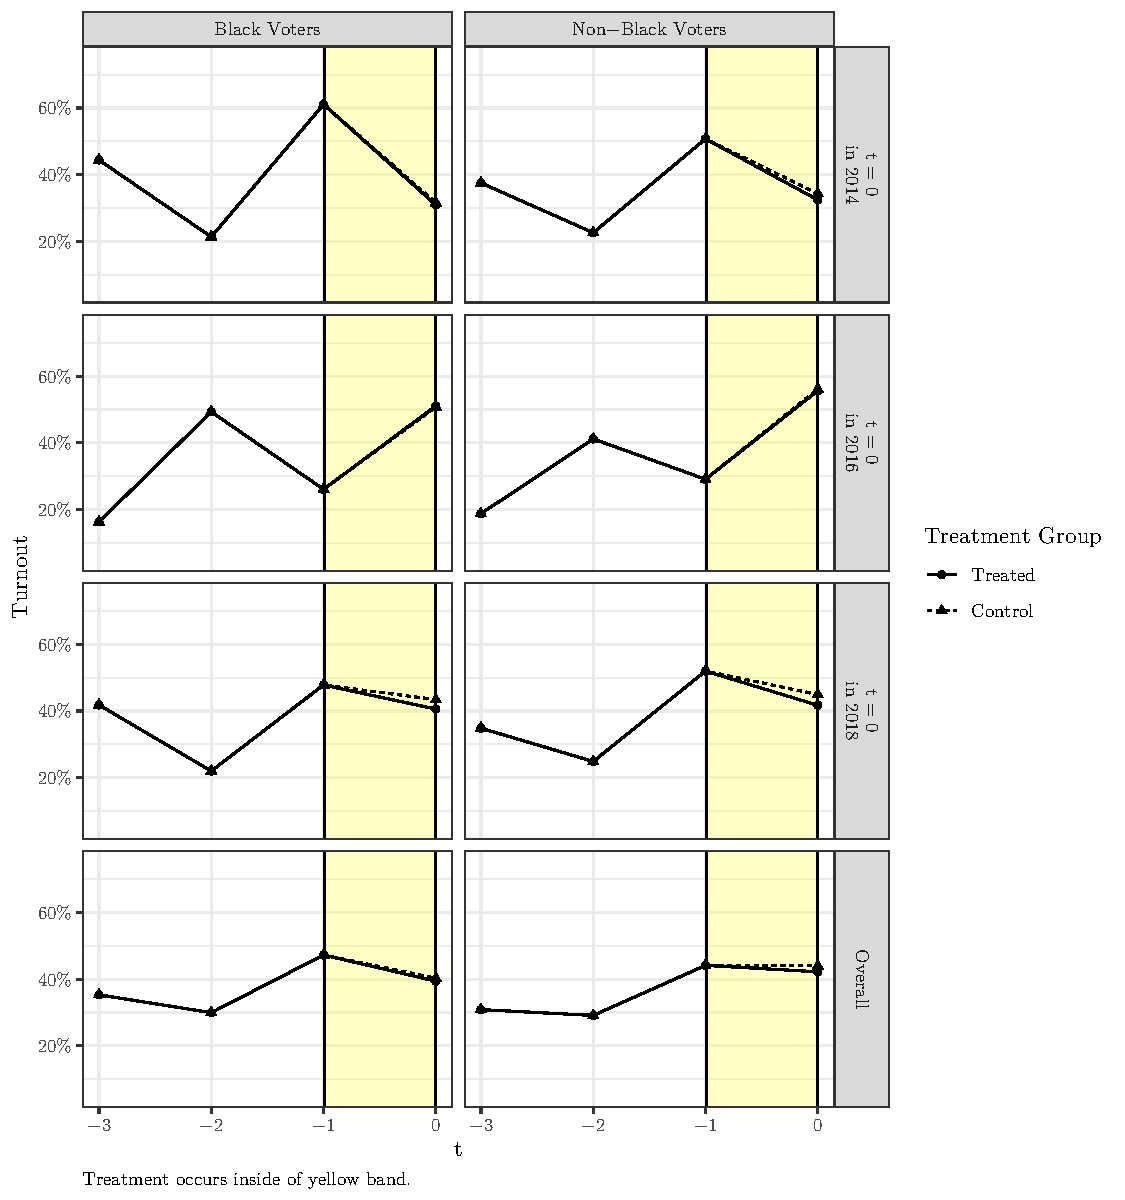
\includegraphics{not_blind_files/figure-latex/did1-1} 

}

\caption{\label{fig:did-1}Effect of Being Ticketed on Turnout}\label{fig:did1}
\end{figure}

\begin{figure}[H]

{\centering 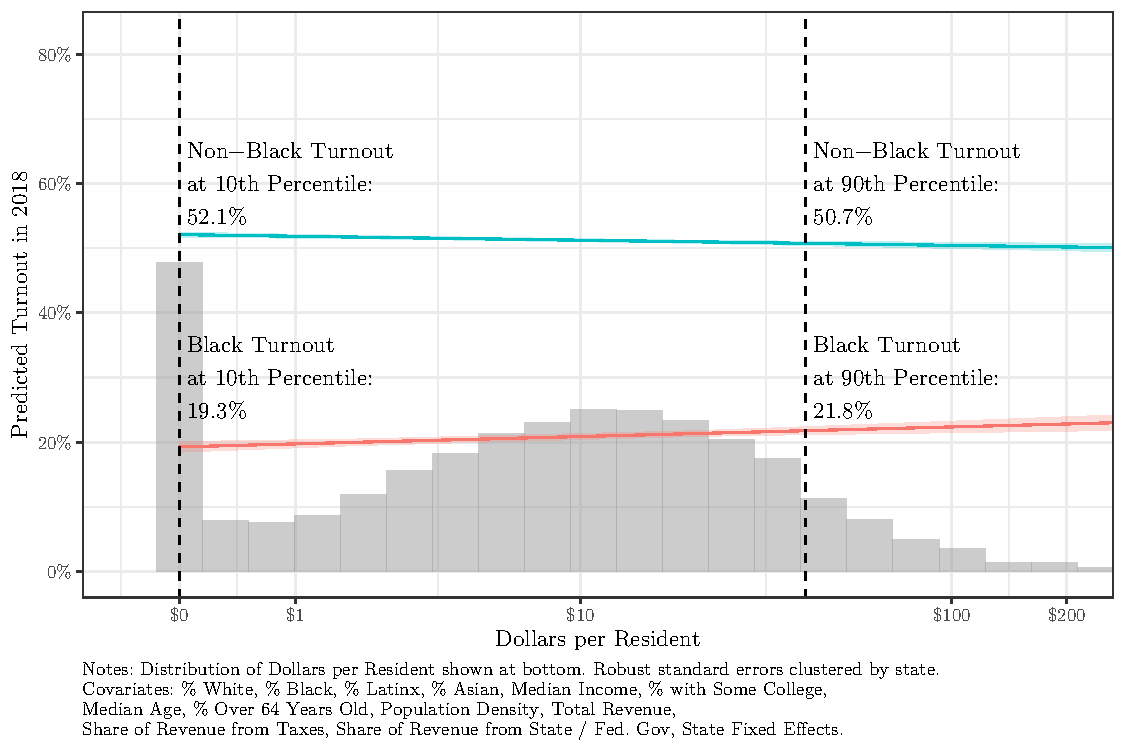
\includegraphics{not_blind_files/figure-latex/cross-18-1} 

}

\caption{\label{fig:mef-2018}Predicted Turnout, 2018}\label{fig:cross-18}
\end{figure}

\begin{figure}[!htpb]

{\centering 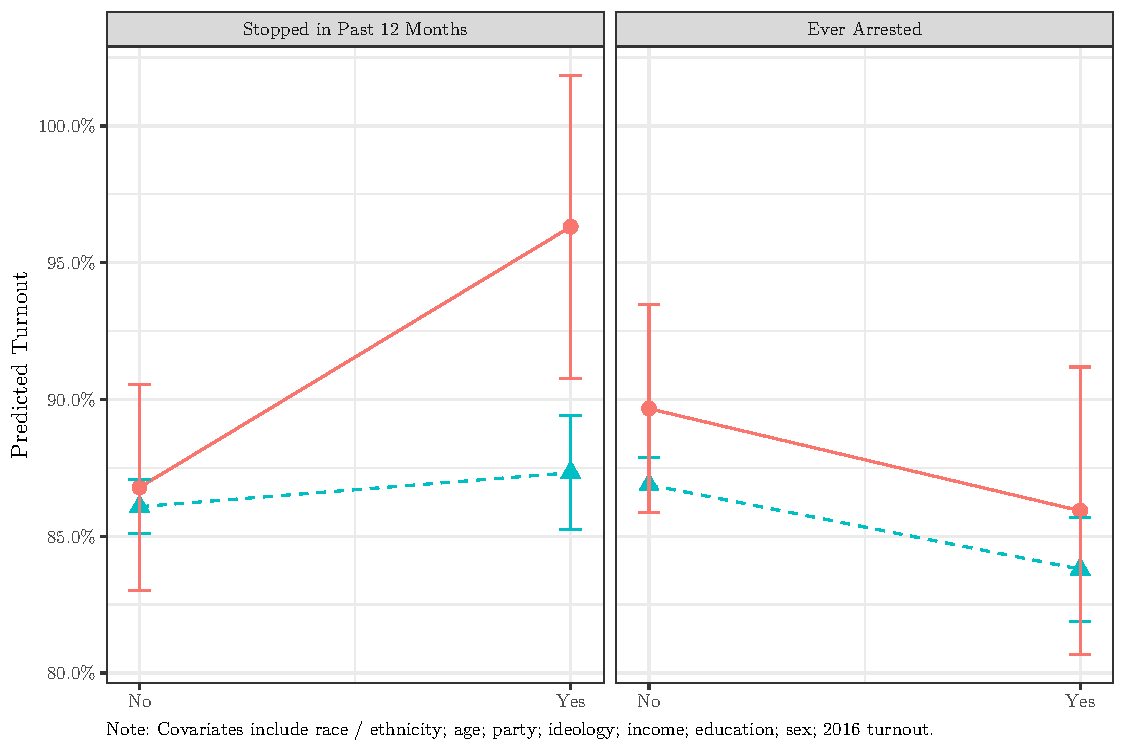
\includegraphics{not_blind_files/figure-latex/anes-cross-1} 

}

\caption{\label{fig:anes}Predicted Turnout, 2020}\label{fig:anes-cross}
\end{figure}

\end{document}
